\section[Theorie: Folgen von SeqAn-Entwurfsentscheidungen]{Theorie über die Entstehung und Auswirkungen von Entwurfsentscheidungen in SeqAn}
\label{sec:gt}

In diesem Abschnitt präsentiere ich meine \gls{gt} über das Zustandekommen von Entwurfsentscheidungen und deren Auswirkungen auf die API-Usability von SeqAn. Dabei beleuchte ich besonders die sich als außerordentlich wichtig herausgestellte \code{apiua://code/-9223372036854775515}\footnote{Zur Erinnerung: Die Kode-/Konzept-/Kategorie-Bezeichner können angeklickt werden. Sie sind verlinkt mit meinen Forschungsdaten. In dieser Darstellung der Theory nenne ich nur einige Phänomene von Konzepten. \textbf{Alle gefundenen Phänomene können in den verlinkten Forschungsdaten nachgelesen werden.} Die Farben geben Aufschluss über die Zusammengehörigkeit von Konzepten und werden durch einen semi-transparenten Kreis (\codebullet{apiua://code/-9223372036854774813}) dargestellt. Ein vollfarbiger Kreis (\codebullet{apiua://code/-9223372036854774814}) markiert besonders wichtige Konzepte. Die Notation wird ausführlich im \sref{sec:notationen} ab Seite \pageref{sec:notationen} beschrieben.}.

\fref{fig:research-gt} visualisiert meine Theorie. Gruppiert sind dabei die gefundenen bzw. entwickelten Konzepte in Form der fünf Hauptkategorien \code{apiua://code/-9223372036854775281}, \code{apiua://code/-9223372036854774893}, \code{apiua://code/-9223372036854774939}, \code{apiua://code/-9223372036854775414} und \code{apiua://code/-9223372036854774875}, wobei \code{apiua://code/-9223372036854775633} die Kernkategorie bildet.

Ich präsentiere meine \gls{gt} in Form einer \textit{Story}, bei der ich auf alle oben genannten Kategorien eingehen werde. Nicht alle Erkenntnisse sind datengetrieben im strengen Sinne der \gls{gtm} zu Stande gekommen. Ein Teil meiner Theorie basiert auf einer technisch-deduktiven Argumentation. Das heißt, habe ich ein Konzept in den Daten erst einmal erkennen können, reichten in solchen Fällen bereits Deduktionsschritte basierend auf existierenden wissenschaftlichen Erkenntnisse, um eben jene Konzepte hinreichend valide zu untermauern. Aussagen mit einem hohen technisch-deduktiven Anteil werden mit \theorybasis{td} ausgezeichnet und sind weniger stark in den aufgezeichneten Daten verankert. Aussagen, die beide Argumentationsstile kombinieren, werden durch \theorybasis{both} gekennzeichnet.

\begin{comment}
\begin{itemize}
%\itemsep1pt\parskip0pt\parsep0pt
  \item[] \code{Konzept}\theorybasis{dd}, das hauptsächlich auf einer datengetriebenen Argumentation basiert
  \item[] \code{Konzept}\theorybasis{td}, das hauptsächlich auf einer technisch-deduktiven Argumentation basiert
  \item[] \code{Konzept}\theorybasis{both}, das sowohl auf einer datengetriebenen als auch auf einer technisch-deduktiven Argumentation basiert
\end{itemize}
\end{comment}


\newgeometry{inner=2cm,outer=1.5cm,top=1.5cm,bottom=1.5cm}
\thispagestyle{empty}
\begin{landscape}
\begin{figure}
  \centering
    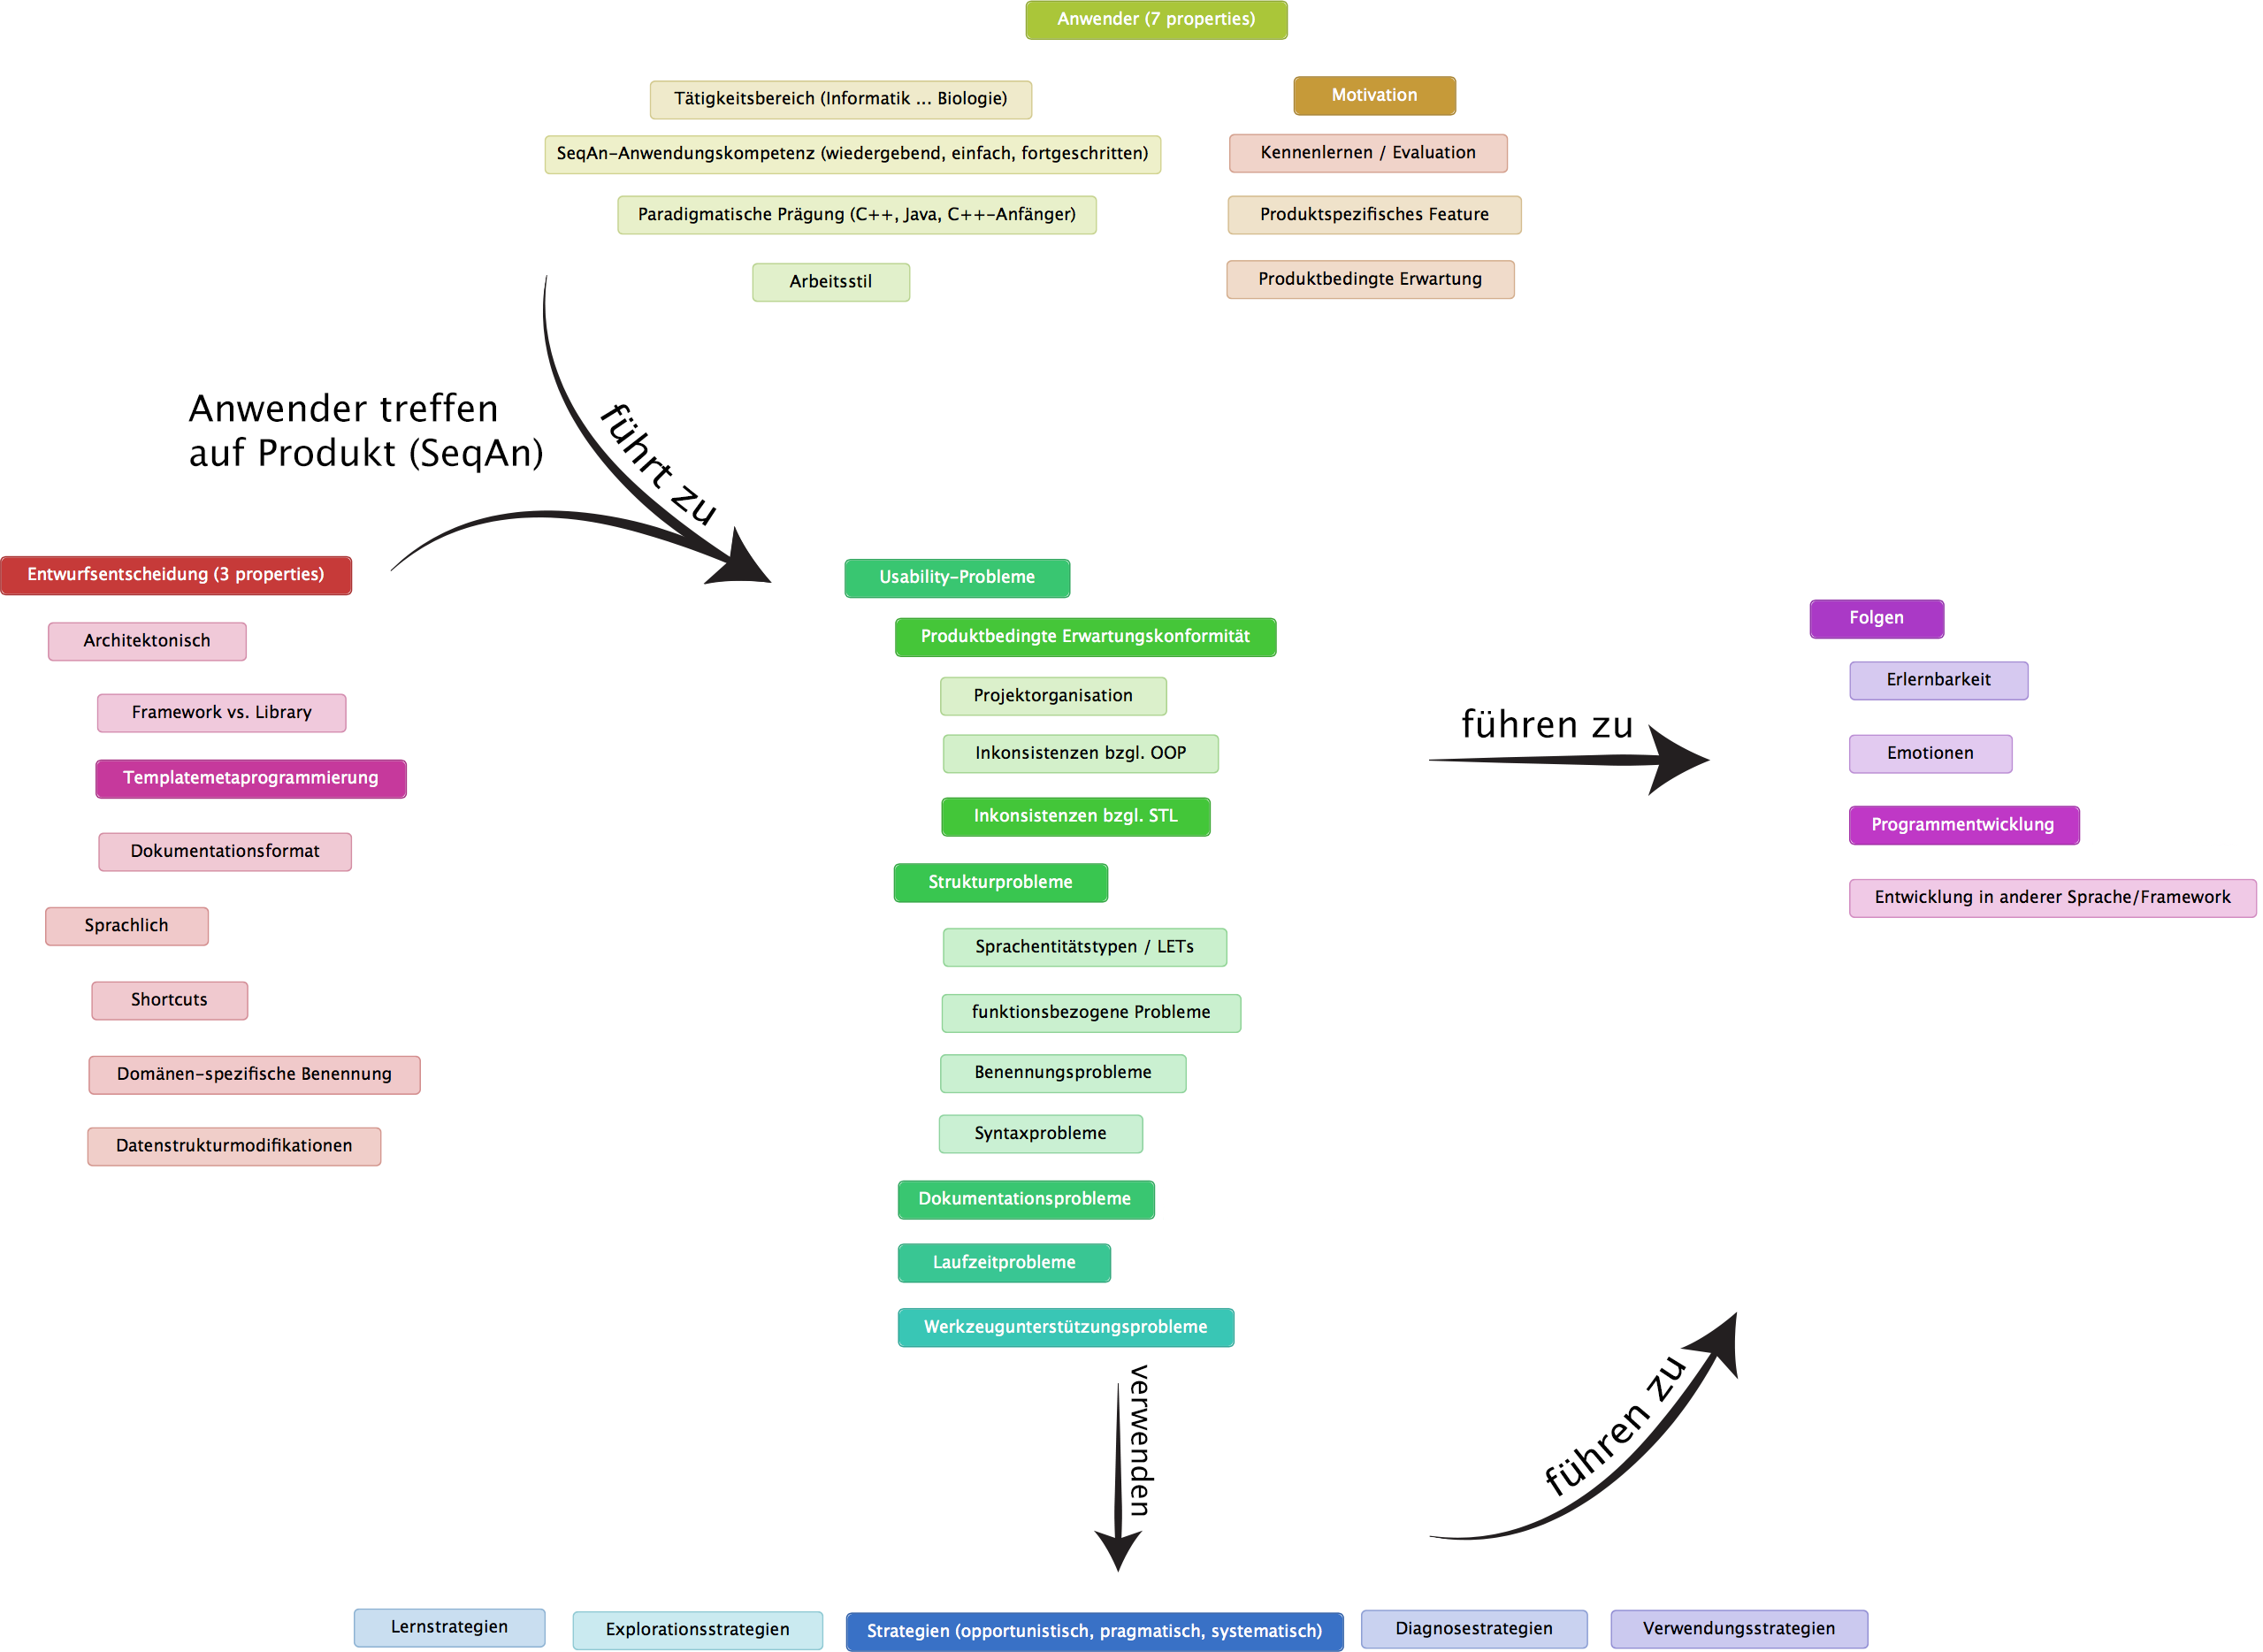
\includegraphics[width=0.8\linewidth]{Figures/research/gt.png}
  \caption[Theorie: Folgen von SeqAn-Entwurfsentscheidungen]{Die Theorie über die Entstehung und Auswirkungen von Entwurfsentscheidungen in SeqAn besteht aus fünf Hauptkategorien, die in Beziehung stehen und dem paradigmatischen Modell ähneln: \code{apiua://code/-9223372036854775281} beschreibt den Entwurf von SeqAn. Mit diesem sind SeqAns \code{apiua://code/-9223372036854774893} konfrontiert, was zu einer Reihe von \code[apiua://code/-9223372036854774939]{Usability-Problemen} führt. Zu Bewältigung kommen häufig \code{apiua://code/-9223372036854775414} zum Einsatz, deren Resultat mit den \code{apiua://code/-9223372036854774875} beschrieben werden.}
  \label{fig:research-gt}
\end{figure}
\end{landscape}
\restoregeometry



\subsection[Anwender]{\code{apiua://code/-9223372036854774893}}

Diese Kategorie beschreibt den Anwender von SeqAn und umfasst alle relevanten Eigenschaften, die zu dessen Charakterisierung notwendig sind. Die API-Anwender zu verstehen ist existenziell notwendig, um die Usability einer API bewerten zu können. Denn Usability-Probleme entstehen erst durch die Verwendung eines Systems durch seine Anwender.

Basierend auf den Ergebnissen meiner \gls{gtm}-Analyse und meiner im \sref{sec:phase1} vorgestellten Beseitigung grober Usability-Probleme, habe ich die folgenden relevanten Eigenschaften entdeckt\footnote{Um Verwunderungen in Bezug auf das von mir verwendete Vokabular auszuräumen: In der Präsentation meiner \gls{gt} verwende ich Verben wie ``beobachten'', ``suchen'' und ``entdecken'', weil dies der Philosophie der \gls{gtm} entspricht \citep[siehe \sref{sec:gtm} und][]{Glaser:1967ts}.}:
\begin{itemize}
  \item[\codebullet{apiua://code/-9223372036854775596}] \textbf{\codetext{apiua://code/-9223372036854775596}} \\
  In welchem Gebiet ist der Anwender vornehmlich tätig? Die Anwenderschaft von SeqAn besteht --- von wenigen Ausnahmen abgesehen --- aus Informatikern, Bioinformatikern und in geringerem Umfang aus Biologen (siehe \sref{sec:results-users}).\citepurl{apiua://code/-9223372036854774893}
  
  Diese Eigenschaft ist wichtig für die weiteren Betrachtungen, da einzelne beobachtete Bioinformatiker\citepurl{apiua://survey/cd/2013-09-18T17:46:55.042+02:00/errorProneness} und Biologen vollständig zu der Gruppe der API-Endanwender gezählt werden. Diese Gruppe zeichnet sich durch einen opportunistischen Arbeitsstil aus.\theorybasis{both}\footnote{Lediglich bei den Cognitive-Dimensions-Fragebögen habe ich nach dem Arbeitsstil gefragt. Dort gab jedoch keiner der Befragten an, einen opportunistischen Arbeitsstil zu haben. Ich gehe davon aus, dass dieser als laienhaft wahrgenommen wird und daher die Frage nicht immer wahrheitsgemäß beantwortet wurde. Tatsächlich kann man in den Programmierfortschritten opportunistisches Verhalten erkennen. In einem Fall\citepurl{https://github.com/bkahlert/seqan-research/blob/master/raw/workshop12/workshop2012-data-20120906/diff/phr0d30hyzmq0xri/phr0d30hyzmq0xri_r00000046_2012-09-05T13-32-11\%2B0200.diff\#L9} wird ein unerwartetes Verhalten einfach durch das manuelle Heraufsetzen einer Zählvariablen umgangen, ohne dass die Dokumentation konsultiert wurde. Ein (anderer) Diskussionsteilnehmer\citepurl{https://github.com/bkahlert/seqan-research/blob/master/raw/workshop12/workshop2012-data-20120906/group-discussions/workshop'12\%20-\%20Interview\%20Gruppendiskussion\%20(2012-09-06T13-01-28\%2B0200).html\#L290} deutet mit seiner Aussage ``a metafunction and this double colon and a type or value behind'', die den Versuch vermissen lässt, Metafunktionen zu verstehen, ebenfalls auf ein opportunistisches Verhalten hin. Diese Beobachtungen, die im \sref{sec:personas} beschriebene Literatur zu \textit{Personas} \citep{clarke:DSP:2007:1080} und die im \sref{sec:euse} beschriebene Literatur zu \textit{\acrlong{euse}} \citep{Ko:2011el} lassen den Schluss zu, dass der opportunistische Arbeitsstil auch unter der SeqAn-Anwenderschaft signifikant vertreten ist.}
  
  \item[\codebullet{apiua://code/-9223372036854775600}] \textbf{\codetext{apiua://code/-9223372036854775600}} \\
  Der Arbeitsstil beschreibt, auf welche Weise Anwender arbeiten. Basierend auf der Arbeit von \cite{clarke:DSP:2007:1080} (siehe \sref{sec:personas}) unterscheide ich den \textit{opportunistischen}, \textit{pragmatischen} und \textit{systematischen} Arbeitsstil. Diese Eigenschaft ist für die Analyse von \code[apiua://code/-9223372036854775414]{Problemlösungsstrategien} relevant.\theorybasis{td}
  
  \item[\codebullet{apiua://code/-9223372036854775494}] \textbf{\codetext{apiua://code/-9223372036854775494}}\label{sec:paradigmatische-pragung} \\
  Von dieser Eigenschaft wurde in der Literatur nach meinem Kenntnisstand noch nicht berichtet. Sie beschreibt, durch welche Programmierparadigmen der Anwender geprägt sein kann.
  
  Erstmalig wurde ich auf diese Eigenschaft aufmerksam, als ich bei der Auswertung der Workshop'12-Fragebögen auf die folgenden Aussagen stieß:
  \begin{itemize}
    \item ``I’m noticing that of the constructs are different from what is common in the STL. This might be justified but it makes it *much* harder to learn.''\citepurl{https://github.com/bkahlert/seqan-research/blob/master/raw/workshop12/workshop2012-data-20120906/feedback/feedback.tsv\#L5}
    \item ``Why don't you use the naming convention (for iterators) used also by STL?''\citepurl{https://github.com/bkahlert/seqan-research/blob/master/raw/workshop12/workshop2012-data-20120906/feedback/feedback.tsv\#L23}
    \item ``Not STL-like. Tries to reinvent STL with global function and it ads a lot of complexity that seems unnecessary.''\citepurl{https://github.com/bkahlert/seqan-research/blob/master/raw/workshop12/workshop2012-data-20120906/feedback/feedback.tsv\#L51}
  \end{itemize}

  
  Ich konnte grob die folgenden zwei Prägungen erkennen: \textit{Java-Objektorientierung} und \textit{C++-/STL-Objektorientierung}. Beiden Prägungen ist gemein, dass sie sich mit der objektorientierten Programmierung befassen. Sie unterscheiden sich jedoch in der Strenge. Während Java streng objektorientiert und sozusagen ``mono-paradigmatisch'' ist, vermischen sich bei der C{}\verb!++!-Objektorientierung verschiedene Paradigmen --- insbesondere das der Templatemetaprogrammierung, welche durch die STL jedoch teilweise durch die Verwendung von \texttt{typedefs} verborgen wird. Beispielsweise ist die \texttt{string}-Klasse\footnote{\url{http://www.cplusplus.com/reference/string/string/}} nichts weiter als ein \mintinline{cpp}{typedef basic_string<char>}.
  
  Diese Prägung habe ich in meiner Datenerhebung nicht explizit, jedoch indirekt über Fragestellungen zu Fertigkeiten mit bekannten Programmiersprachen erfragt. In Zusammenhang mit der Nennung verschiedener Usability-Probleme war es häufig nicht schwierig, auf die paradigmatische Prägung zu schließen. Gab ein Anwender\citepurl{https://github.com/bkahlert/seqan-research/blob/master/raw/workshop12/workshop2012-data-20120906/feedback/feedback.tsv\#L7} beispielsweise an, die besten Kenntnisse in Bezug auf Java zu haben und bezeichnete sich dieser auch noch als Java-Entwickler, wurde klar, dass er eine \code[apiua://code/-9223372036854775494]{Java-objektorientierte Prägung} besaß.
  
  Diese Eigenschaft ist ursächlich für eine Reihe von \code[apiua://code/-9223372036854774939]{Usability-Problemen}.
  
  \item[\codebullet{apiua://code/-9223372036854774938}] \textbf{\codetext{apiua://code/-9223372036854774938}} \\
  Diese Eigenschaft beschreibt, in welcher Form SeqAn eingesetzt werden kann. Zu beobachten war, dass Anwender SeqAn entweder zur Implementierung von \textit{Hilfsprogrammen}\citepurl{apiua://code/-9223372036854775587} oder zur Entwicklung einer ganzen \textit{Pipeline}\footnote{Für die Sequenzanalyse werden häufig mehrere Phasen durchlaufen. Dazu gehört u.a. die Vorbereitung der Daten (\textit{Proprocessing}) und die Visualisierung der Analyseergebnisse. Die technische Aneinanderreihung dieser Phasen wird häufig als \textit{Pipeline} bezeichnet.}\citepurl{apiua://code/-9223372036854775598} nutzten. Dies wurde auch in persönlichen Gesprächen mit den Workshop-Teilnehmer bestätigt.%\footnote{Tatsächlich wird SeqAn auch innerhalb von Abschlussarbeiten verwendet, worauf allerdings nicht mein Fokus lag.}
  
  Die Relevanz dieser Eigenschaft wird weiter unten deutlich.
  
   
  
  \item[\codebullet{apiua://code/-9223372036854775446}] \textbf{\codetext{apiua://code/-9223372036854775446}} \\
  Diese Eigenschaft beschreibt, welche Erfahrung Anwender im Gebrauch von SeqAn besitzen können. Differenziert wird diese Eigenschaft in Anlehnung an die verschiedenen Tutorial-Übungsaufgaben-Schwierigkeitsgrade, die im \sref{sec:tutorials-improve} beschrieben und für meine Zwecke hinreichend validiert sind\theorybasis{both}. Sie lauten:
  
  \begin{description}
    \item[Lernen] Der Anwender lernt SeqAn erst kennen und kann bestenfalls den SeqAn-Anwendungscode so weit verstehen, dass er einfache Anpassungen vornehmen kann. 
    \item[Anwendung] Der Anwender beherrscht SeqAn hinreichend, um existierenden Code neu komponieren und mehrzeilige Anwendungen selbstständig implementieren zu können.
    \item[Beherrschung] Der Anwender verfügt über genügend Kenntnisse, dass er selbstständig SeqAn-Anwendungen für seinen eigenen Bedarf schreiben kann. 
  \end{description}
  
  Meine Betrachtungen beschränken sich weitgehend auf Anwender, die SeqAn nicht beherrschen und dürften für Anwender mit guter SeqAn-Beherrschung nur geringe Gültigkeit haben.
  
  \item[\codebullet{apiua://code/-9223372036854775599}] \textbf{\codetext{apiua://code/-9223372036854775599}} \\
  Die Eigenschaft befasst sich mit den Gründen, aus denen sich Anwender mit SeqAn befassen. Diese Eigenschaft verfügt über die folgenden Untereigenschaften:
  
  \begin{itemize}
    \item[\codebullet{apiua://code/-9223372036854775407}] \textbf{\codetext{apiua://code/-9223372036854775407}} \\
    Es handelt sich hierbei um eine boolesche Eigenschaft. Sie gibt Auskunft darüber, ob potentielle Anwender SeqAn zunächst kennen lernen wollen. Dieses Kennenlernen kann zielgerichtet sein. In diesem Fall spreche ich von Evaluation. Die Anwender gaben wenig überraschend an, SeqAn für die Sequenzanalyse zu verwenden und SeqAns Eignung zu diesem Zweck überprüfen zu wollen. Ein Anwender\citepurl{apiua://code/-9223372036854775547} hatte besonders konkrete Vorstellungen. Er hatte bereits eine entsprechende Pipeline in der Programmiersprache C entwickelt und wollte prüfen, inwiefern er diese nach SeqAn portieren kann, um von SeqAns \code[apiua://code/-9223372036854775552]{Performance-Eigenschaft} profitieren zu können.
    
    \item[\codebullet{apiua://code/-9223372036854774827}] \textbf{\codetext{apiua://code/-9223372036854774827}} \\
    Diese Eigenschaft beschreibt Erwartungen, die beim Anwender durch das Produkt --- also durch SeqAn --- geweckt werden können. Wie noch weiter unten erläutert wird, weckt SeqAn die folgenden Erwartungen:
    
    \begin{itemize}
      \item[\codebullet{apiua://code/-9223372036854774830}] \textbf{\codetext{apiua://code/-9223372036854774830}} \\
      Erwartung, dass es sich bei SeqAn um eine Softwarebibliothek handelt, die in das eigene Projekt eingebunden werden kann. Interessanterweise wurde ich auf diese Erwartung nur durch persönliche Gespräche --- vielfach --- aufmerksam. In meinen technisch erfassten Daten ist diese Erwartung nicht ohne Weiteres zu finden. Verantwortlich mache ich dafür das Umfeld, in dem die Datenaufzeichnungen stattfanden. Diese waren nämlich stets moderiert (Workshop bzw. Projektseminar, siehe \sref{sec:rahmenbedingungen}) und hatten nicht den Fokus auf die Integration von SeqAn in einem eigenen Projekt, sondern auf das Erlernen von SeqAn in einer vergleichsweise praxisfremden Umgebung.\theorybasis{both}
      
%      \item[\codebullet{apiua://code/-9223372036854775568}] \textbf{\codetext{apiua://code/-9223372036854775568}} \\
%      Erwartung, dass SeqAn für ein großes Funktionsspektrum verfügt.
      
      \item[\codebullet{apiua://code/-9223372036854775298}] \textbf{\codetext{apiua://code/-9223372036854775298}} \\
      Erwartung, dass die mit SeqAn entwickelten Anwendungen besonders schnell sind.\citepurl{apiua://survey/cd/2013-09-19T11:51:16.616+02:00/provisionality}
      
      \item[\codebullet{apiua://code/-9223372036854775311}] \textbf{\codetext{apiua://code/-9223372036854775311}} \\
      Erwartung, dass SeqAn einfach in der Anwendung ist.\citepurl{apiua://survey/cd/2013-09-19T11:51:16.616+02:00/roleExpressiveness}\citepurl{apiua://survey/cd/2013-09-18T17:44:46.060+02:00/learningStyle}
    \end{itemize}
        
    \item[\codebullet{apiua://code/-9223372036854774826}] \textbf{\codetext{apiua://code/-9223372036854774826}} \\
    Die Eigenschaft unterscheidet sich von \codebullet{apiua://code/-9223372036854774827}{produktbedingen Erwartungen} in dem Grad der Gewissheit. Sie beschreibt keine Erwartung, sondern das Wissen um eine Eigenschaft und betrifft hauptsächlich Anwender, die sich bereits von den Vorzügen der folgenden Eigenschaft überzeugen konnten und aus diesem Grund SeqAn einsetzen.
    
    \begin{itemize}
%      \item[\codebullet{apiua://code/-9223372036854775297}] \textbf{\codetext{apiua://code/-9223372036854775297}} \\
%      Wissen um das große Funktionsspektrum von SeqAn.
      
      \item[\codebullet{apiua://code/-9223372036854775552}] \textbf{\codetext{apiua://code/-9223372036854775552}} \\
      Wissen um die hohe Performance von mit SeqAn entwickelten Programmen.\citepurl{apiua://survey/cd/2013-09-18T17:50:13.425+02:00/mainPurpose}\citepurl{apiua://groupDiscussion/workshop\%2712+-+Interview+Gruppendiskussion+\%282012-09-06T13-01-28\%2B0200\%29.html/li/1}
    \end{itemize}
    
    Die auffälligste Beobachtung ist, dass in keiner meiner Datenerhebungen ein Proband von der Benutzerfreundlichkeit von SeqAn berichtete, obwohl es die dazugehörige Erwartung gibt.
  \end{itemize}  
  
\end{itemize}




\subsection[Entwurfsentscheidungen]{\code[apiua://code/-9223372036854775281]{Entwurfsentscheidungen}}
\label{sec:gt-entwurfsentscheidungen}

SeqAn wurde von Andreas Gogol-Döring im Rahmen seiner Dissertation ``SeqAn --- A Generic Software Library for Sequence Analysis'' \citep{GogolDoring:2009vz} entwickelt. Auf der Grundlage seiner Arbeit habe ich die Kategorie \code[apiua://code/-9223372036854775281]{Entwurfsentscheidungen} erarbeitet, welche alle Entscheidungen auf Seiten der API-Entwickler beschreiben können soll, die den Entwurf von SeqAn prägen. Unterschieden wird dabei grundsätzlich in \code[apiua://code/-9223372036854774919]{architektonische} und \code[apiua://code/-9223372036854774918]{sprachliche Entwurfsentscheidungen}. Diese Unterscheidung stammt von \cite{Stylos:2007ip} (siehe \fref{fig:APIDesignDecisions} auf Seite \pageref{fig:APIDesignDecisions}).

Entwurfsentscheidungen können mit Hilfe der folgenden Eigenschaften charakterisiert werden:

\begin{itemize}
  \item[\codebullet{apiua://code/-9223372036854774864}] \textbf{\codetext{apiua://code/-9223372036854774864}} \\
  Diese Eigenschaft beschreibt das Ziel, mit der eine Entwurfsentscheidung getroffen wurde. Entdeckte Ziele sind \textit{Performance} und \textit{Usability}. Andere Ziele wie \textit{Simplizität} habe ich unter \textit{Usability} subsummiert.
  
  \item[\codebullet{apiua://code/-9223372036854774942}] \textbf{\codetext{apiua://code/-9223372036854774942}} \\
  Diese Eigenschaft beschreibt die Motivation der Entwurfsentscheidung. Dabei kann es sich entweder um die Absicht handeln, das erklärte Ziel zu erreichen (\textit{Zielverfolgungsabsicht}) oder um eine \textit{notwendige Folgeentscheidung}, die sich aus einer vorangegangenen Entwurfsentscheidung ergibt. Ist Letzteres der Fall, so kann es ein Entwurfsentscheidungsziel geben --- und zwar dann, wenn der API-Entwickler beispielsweise etwas kompensieren muss. Die weiter unten besprochene \code[apiua://code/-9223372036854775281]{Folge-Entwurfsentscheidung} \code{apiua://code/-9223372036854775412} diente dazu, die Usability zu steigern, indem Polymorphie ermöglicht wurde. Dieser Schritt war jedoch nur notwendig, weil durch den Einsatz von \code{apiua://code/-9223372036854775515} und den Verzicht auf objektorientierte Programmierung Polymorphie zunächst nicht mehr nutzbar gewesen ist. 
  
  \item[\codebullet{apiua://code/-9223372036854774839}] \textbf{\codetext{apiua://code/-9223372036854774839}} \\
  Diese Eigenschaft beschreibt die Art, wie die Entwurfsentscheidung zustande kam bzw. umgesetzt wurde. Die entsprechende Dimension umfasst dabei das Spektrum von \textit{implizit} bis \textit{explizit-empirisch}.
  
  \begin{description}
    \item[Implizite] Entwurfsentscheidungen sind solche, die unbewusst getroffen wurden. Diese Art ist häufig anzutreffen, wenn es sich um eine notwendige Folgeentscheidung handelt. In dieser Konstellation hat der API-Entwickler nicht erkannt, dass er gerade eine Entwurfsentscheidung trifft, was tendenziell ein weniger vorhersagbares Ergebnis bedingt.
    \item[Explizite-intuitive] Entwurfsentscheidungen sind solche, die zwar erkannt wurden, jedoch lediglich intuitiv getroffen wurden. Implizite und explizit-intuitive Entscheidungen bezeichne ich auch als \code{Bauchgefühlentscheidung}. \label{sec:bauch-usability}
    \item[Explizite-argumentative] Entwurfsentscheidungen unterscheiden sich von explizit-intuitiven Entwurfsentscheidungen dadurch, dass sie argumentiert werden. Als Argumente dienen u.a. Erfahrungen des API-Entwicklers oder Entwurfsentscheidungen, die von Dritten in anderen Produkten getroffen und adaptiert wurden.
    \item[Explizite-empirische] Entwurfsentscheidungen haben die höchste Wahrscheinlichkeit, das Entscheidungsziel zu erreichen. Die Wirksamkeit derartiger Entwurfsentscheidungen wird vom Entscheider empirisch belegt. Der empirische Wirkungsnachweis kann dabei selbst erbracht werden oder auf empirisches Untersuchen in verwandten Arbeiten fußen. 
  \end{description}
  
  Bei der vorgestellten Unterteilung handelt es sich um eine Dimension mit zwei Extremen und erlaubt viele Schattierungen. So sind die Grenzen zwischen den expliziten Entscheidungsgrundlagen fließend --- je nachdem, wie solide die Argumentation ist.
  
  Implizite Entwurfsentscheidungen sind weniger differenziert, denn das Fehlen der Explikation der Entscheidungsgrundlage lässt keine zuverlässige Unterscheidung zu.
\end{itemize}

\bigskip

In Bezug auf \code[apiua://code/-9223372036854775281]{Entwurfsentscheidungen} kann SeqAn also wie folgt beschrieben werden:

SeqAn wurde als quelloffene Softwarebibliothek (\textit{Library}) entworfen, welche auf C{}\verb!++! basiert und zum ultimativen \code{apiua://code/-9223372036854774864} die Geschwindigkeit (\textit{Performance}) von mit SeqAn entwickelten Programmen hatte. Ein weiteres \codetext{apiua://code/-9223372036854774864} war die Benutzerfreundlichkeit (\textit{Usability}) von SeqAn.

Diese Beschreibung, welche sich auch auf der SeqAn-Website\footnote{\url{http://www.seqan.de}} befindet, weckt auf \code[apiua://code/-9223372036854774893]{Anwenderseite} vier \code[apiua://code/-9223372036854774827]{produktbedingte Erwartungen}, von denen drei nicht erfüllt werden. Diese bezeichne ich informell gerne auch als \textit{die drei Urlügen / -täuschungen}. Die im Folgenden vorgestellten, unerfüllten \code[apiua://code/-9223372036854774827]{produktbedingten Erwartungen} bzw. \textit{Urlügen} basieren auf meinen Analysen der in \sref{sec:datenerhebung} vorgestellten Datenquellen, sowie der im vorherigen Absatz genannten Dissertation \citep{GogolDoring:2009vz} und einem längeren Telefonat mit Andreas Gogol-Döring \citep{GogolDoring:5iYhf2VJ}:

\begin{description}
  \item[1. Framework statt Softwarebibliothek]\label{sec:lie-library}\label{sec:library-vs-framework} (\code{apiua://code/-9223372036854774830}) \\
  SeqAn sollte eine Library sein, wurde jedoch als Framework entwickelt.
  
  Der Unterschied besteht in der Art, wie das ``architektonische Skelett'' der entwickelten Anwendungen durch die Library bzw. das Framework vorgegeben wird. Bei einer Library ist der API-Anwender weitgehend unbeeinflusst --- er bindet die durch die Library bereitgestellte Funktionalität lediglich ein. Bei einem Framework wird die Struktur der entwickelten Anwendungen weitgehend von dem Framework vorgegeben. \citep{Fairbanks:2006jw}
  
  Diese Form der Implementierung wird durch die \code[apiua://code/-9223372036854774919]{architektonische Entwurfsentscheidung} \code{apiua://code/-9223372036854775215} erfasst. Dabei handelt es sich nach meiner Einschätzung um eine \textit{implizite} Entscheidung, denn Gogol-Döring lässt in seiner Dissertation kein Bewusstsein vermuten, dass die folgenden Beobachtungen de facto zur Implementierung eines Frameworks führen\theorybasis{td}:
  
  \begin{itemize}
    \item SeqAn verwendet das plattformübergreifende Build-System \textit{CMake}\footnote{\url{http://www.cmake.org}}. Das hat zur Folge, dass SeqAn-Anwender Programme nur innerhalb dieses Systems entwickeln können. Eine Einbindung von SeqAn in das eigene C{}\verb!++!-Projekt --- durch Inkludierung einer entsprechenden Header-Datei --- ist \textit{nicht} vorgesehen.
    \item Die SeqAn-Entwickler nutzen Vorausdeklarationen (\textit{forward declarations}), um API-interne Abhängigkeiten aufzulösen. Diese werden durch ein, in das Build-System integriertes Python-Skript bei jedem Kompilieren automatisch generiert, was die Komplexität von Vorausdeklarationen verringert. Ein SeqAn-Anwender müsste für den Gebrauch von SeqAn als Library dieses Skript selbst ausführen.
    \item SeqAn verwendet eine dreigliedrige Organisation. Der \textit{Core} umfasst dabei alles, was zu SeqAn gehört. \textit{Extras} beinhaltet funktionale Erweiterungen, die weitgehend auf die Ergebnisse von Abschlussarbeiten zurückgehen. Ist ein Extra von großer Relevanz und genügt es nicht näher spezifizierten Qualitätsanforderungen, wird es in den Core aufgenommen. Schließlich gibt es noch die \textit{Sandboxes}. Jeder SeqAn-Anwender muss mit Hilfe eines Python-Skripts eine Sandbox erstellen. Innerhalb seiner Sandbox wiederum werden durch abermalige Python-Skript-Aufrufe \textit{Apps} erzeugt. Dabei handelt es sich um ein Skelett zur Entwicklung von SeqAn-Anwendungen. Die Verwendung des Python-Skripts ist obligatorisch, denn es erweitert das Build-System so, dass die selbst entwickelten SeqAn-Anwendungen / -Apps auch kompiliert werden können.
  \end{itemize}
  
  Aus diesen Gründen, ist SeqAn keine Library, sondern ein Framework. SeqAn kann nicht ohne weiteres in eigene Entwicklungsprojekte eingebunden werden, was in seiner Verwendung von CMake, dem Gebrauch von Vorausdeklarationen und der Vorgabe der Projektstruktur begründet ist. Damit wird massiv die oben beschriebene \code[apiua://code/-9223372036854774830]{Libraryerwartung} verletzt. Außerdem wird die \code[apiua://code/-9223372036854774938]{SeqAn-Einsatzform} eingeschränkt, wenn der Gebrauch als Library vorgezogen wird. Mehrere Workshop-Teilnehmer\citepurl{apiua://code/-9223372036854774830} gaben in mündlichen Gesprächen an, dass sie die Framework-Gestalt von SeqAn für inakzeptabel halten, da sie bereits ein eigenes Build-System betreiben und ein Wechsel nicht in Frage kommt. Dieses praxisrelevanten Äußerungen legen nahe, dass SeqAns Framework-Gestalt in der Praxis für viele potentielle Anwender ein Problem darstellt.\theorybasis{both}
  
  \item[2. Programmierparadigma]\label{sec:lie-oop} (\code{apiua://code/-9223372036854774809}) \\ 
  SeqAn nutzt als Programmiersprache C{}\verb!++!. Dies weckt Erwartungen, die im Konflikt zur anwenderseitigen \code[apiua://code/-9223372036854775494]{paradigmatischen Prägung} stehen können und u.a. folgende Wortmeldungen zur Folge haben:
  
  \begin{itemize}
    \item Ein Anwender mit einer \code[apiua://code/-9223372036854775494]{Java-Objektorientierungsprägung} bezeichnete SeqAn als ``Vergewaltigung der OO-Programmierung''\citepurl{apiua://survey/2011-09-14-T15:23:17.211+02:00}.
    \item Ein Anwender mit einer \code[apiua://code/-9223372036854775494]{C{}\texttt{++}-/STL-Objektorientierungsprägung} sagte: ``If SeqAn [just] had the same way of doing things like the STL''\citepurl{apiua://groupDiscussion/workshop\%2712+-+Interview+Gruppendiskussion+\%282012-09-06T13-01-28\%2B0200\%29.html/li/9}.
    \item Ein Anwender sagte allgemein im Zusammenhang mit der \code{apiua://code/-9223372036854775515}: ``[It's] not clear why you have to go through all this pain''\citepurl{apiua://groupDiscussion/workshop\%2712+-+Interview+Gruppendiskussion+\%282012-09-06T13-01-28\%2B0200\%29.html/li/14}.
  \end{itemize}
  
  Offenbar ``tickt'' SeqAn also anders, als es seine Anwender erwarten. Gogol-Döring traf die architektonische Entwurfsentscheidung, für die Entwicklung von SeqAn keine klassische Objektorientierung, sondern das Programmierparadigma \code{apiua://code/-9223372036854775515} zu verwenden.
  
  In seiner Dissertation stellt Gogol-Döring die Vorzüge der Templatemetaprogrammierung dar, ohne jedoch die Nachteile der Objektorientierung näher zu beleuchten. In dem Telefonat mit Gogol-Döring \citep{GogolDoring:5iYhf2VJ} erfragte ich diese:
  \begin{itemize}
    \item Gogol-Döring teilte mir mit, dass er kein Freund von objektorientierter Programmierung (OOP) sei. Als Beispiel nannte er, dass die Implementierung symmetrischer Operationen, wie der Addition, in der OOP auf eine ihm ``befremdliche'' Art gelöst würden --- nämlich durch Memberfunktionen und nicht durch ``symmetrische'', globale Funktionen.
%    \item -- Leere Basisklassen bekommen bei manchen Compilern ein Junk-Byte, weil leere Klassen nicht gehen $\rightarrow$ Speicherverbrauch
    \item Hauptargument für die Verwendung der Templatemetaprogrammierung war jedoch die dadurch hohe zu erreichende Performance. Zum Erreichen von Polymorphie werden in C{}\verb!++! virtuelle Funktionen benötigt. Welche Funktion tatsächlich zur Ausführung kommt, wird zur Laufzeit bestimmt --- und das kostet Rechenzeit (\textit{virtual lookup overhead}). Um die Bestimmung der aufzurufenden Funktion performance-steigernd zur Kompilierzeit zu berechnen (\textit{static binding}) und gleichzeitig Polymorphie zu erlauben, traf der SeqAn-Autor die Entscheidung, \code{apiua://code/-9223372036854775412} (\textit{Template Subclassing}) zu verwenden.
    \item Gogol-Döring experimentierte mit Möglichkeiten, eine hohe Performance mit Hilfe der OOP zu erreichen. Dies gelang ihm jedoch nicht.
%-- keine Shims-Funktionalität (Bereitstellung der Funktionalität für fremde Datentypen, z.B. STL-String)
  \end{itemize}
  
%  In Anbetracht dieser Argumentation und der seiner Dissertation kann man zusammenfassen, dass Gogol-Döring sich --- auch aus Präferenzgründen --- gegen OOP und für \code{apiua://code/-9223372036854775515} entschieden hat. Dabei handelt es sich um eine \textit{explizite-empirische} \code{apiua://code/-9223372036854775281}, denn der Autor konnte zeigen, dass er damit tatsächlich das \code{apiua://code/-9223372036854774864} \textit{Performance} erreichen konnte. Jedoch führt dieser Ansatz zu einer Reihe weiter unten beschriebener \code{apiua://code/-9223372036854774939}.
  
  \item[3. Usability]\label{sec:lie-usability} (\code{apiua://code/-9223372036854775311}) \\
  Gogol-Döring beschreibt als weiteres Entwurfsziel die \textit{Usability}. Um dies zu erreichen, entschloss sich der Autor zu der ebenfalls architektonischen Entwurfsentscheidung \code{apiua://code/-9223372036854775579}\footnote{Tatsächlich verfolgte Gogol-Döring mit der \code[apiua://code/-9223372036854775579]{Generischen Programmierung}, neben der \textit{Usability}, weitere Ziele wie \textit{Simplizität}, \textit{Generalisierbarkeit} und \textit{Erweiterbarkeit}. Für den Zweck meiner Arbeit reicht die zusammenfassende Betrachtung \textit{Usability}.}. Generische Funktionen lösen Probleme allgemeingültig. Kann ein Problem für bestimmte Eingaben effizienter gelöst werden (z.B. bei der Sortierung), kann eine spezialisierte Funktion implementiert werden. Der Compiler wählt beim Kompilieren die spezialisierteste Implementierung aus und bindet diese Funktion statisch, was die Performance von SeqAn sicherstellt \citep[Details siehe][]{GogolDoring:2009vz}.
% - open-closed principle
%  - neue Funktionalität ohne Codeänderung
%  - e.g. neue Spezialisierung, neue Funktionen
%  - Auslagerung in weitere header Dateien
  
  Ungünstigerweise werden generische Funktionen nicht als Memberfunktionen, sondern als globale Funktionen implementiert. Damit entfällt jedoch technisch die immer noch existierende inhaltliche Zusammengehörigkeit von Funktionen, was in der OOP durch die Klassenzugehörigkeit implementiert wird. Üblicherweise erwartet eine generische Funktion ihr \textit{Hauptobjekt} als erstes Argument. Schreibt man in OOP also \mintinline{java}{myString.length()}, lautet der gleiche Aufruf in SeqAn \mintinline{cpp}{length(myString)}. In SeqAn wird die inhaltliche Zusammengehörigkeit von Funktionen als \textit{global function interface} bezeichnet und nur noch in der Dokumentation beschrieben, was insbesondere \code{apiua://code/-9223372036854774819} behindert.
  
  Durch die globale Implementierung von generischen Funktionen, firmieren unterschiedliche Funktionen unter dem gleichen Namen im globalen Namespace. Entsprechend variabel ist auch deren Rückgabetyp. Den korrekten Rückgabetyp zu ermitteln, ist mühsam und fehlerträchtig. Um u.a. dieses Problem zu lösen, wurde die Entwurfsentscheidung \code{apiua://code/-9223372036854775514} getroffen. Dabei handelt es sich um Funktionen, die nicht zur Laufzeit, sondern zur Kompilierzeit ausgeführt werden. Sie werden dazu verwendet, den korrekten Typ für die Rückgabe einer generischen Funktion zu berechnen. Syntaktisch ähneln Metafunktionen allerdings Klassen, da Metafunktionen in SeqAn ebenfalls mit einem Großbuchstaben beginnen\theorybasis{td}. Da die SeqAn-Anwender über eine unpassende \code{apiua://code/-9223372036854775494} verfügen, führt dies zu \code[apiua://code/-9223372036854774939]{Usability-Problemen}, die weiter unten erläutert werden.
  
  \code{apiua://code/-9223372036854775579} und \code{apiua://code/-9223372036854775514} sind im Falle von SeqAn \textit{explizite-argumentative} \code[apiua://code/-9223372036854775281]{Entwurfsentscheidungen} mit dem \code{apiua://code/-9223372036854774864} \textit{Usability}. Ein empirischer Beleg für die Wirksamkeit der Entscheidungen fehlt. Stattdessen wird die Wirksamkeit nur unzureichend argumentativ an drei Stellen seiner Dissertation \citep{GogolDoring:2009vz} erbracht:
  \begin{itemize}
    \item In Unterkapitel 14.1 argumentiert der Autor, dass SeqAn lediglich eine geringe Anzahl von Techniken kombiniert, von denen jede nur eine begrenzte Komplexität (``limited complexity'') aufweist. Gleichzeitig räumt er aber ein, dass sein Ansatz als unüblich von den meisten Programmierern empfunden werden könnte und Fehlerausgaben der Compilers ``ziemlich'' schwer verständlich sind. % Darüber hinaus beschreibt er die durch \code{apiua://code/-9223372036854775412} ermöglichte Polymorphie als Vereinfachung.
    In dieser Betrachtung unterschätzt Gogol-Döring im erheblichen Maß die Auswirkungen seines Entwurfs.
    \item In Unterkapitel 14.2 argumentiert der Autor, dass der erfolgreiche Einsatz von SeqAn im Rahmen von Arbeiten innerhalb der Bioinformatik-Arbeitsgruppe die Usability bestätigt. Allerdings ignoriert er dabei, dass die meisten Anwender die Entwicklung von SeqAn miterlebten/-gestalteten und sich bei Problemen, direkt an den Autoren wenden konnten.
    \item In Kapitel 15 demonstriert Gogol-Döring die Re-Implementierung der Basisfunktionalität eines Bioinformatik-Werkzeugs. Damit stellt er allerdings lediglich unter Beweis, dass SeqAn für ihn selbst benutzbar ist. 
  \end{itemize}
  
%  Zusammenfassend kann man sagen, dass Gogol-Döring den Fehler begangen hat, die Usability von SeqAn nicht ausreichend belegt zu haben. Der größte Mangel besteht darin, die Anwender von SeqAn nicht ausreichend berücksichtigt zu haben.
  
  Die in Kapitel 15 angeklungene \code{Bauchgefühl-Usability} setzt sich in sämtlichen \code[apiua://code/-9223372036854774918]{sprachlichen Entwurfsentscheidungen} fort, d.h. all diese Entscheidungen sind \textit{implizit} oder \textit{explizit-intuitiv} --- werden also gar nicht oder nur intuitiv begründet:
  \begin{itemize}
    \item[\codebullet{apiua://code/-9223372036854775611}] \textbf{\codetext{apiua://code/-9223372036854775611}} \\
    Hierbei handelt es sich um C{}\verb!++!-\texttt{typedefs}, die eine einfachere Schreibweise von häufigen Templatespezialisierungen bereitstellen sollen. Beispiel: Das Shortcut \mintinline{cpp}{DnaString} kann anstelle von \mintinline{cpp}{String<Dna>} verwendet werden.
    
    \item[\codebullet{apiua://code/-9223372036854774848}] \textbf{\codetext{apiua://code/-9223372036854774848}} \\
    In SeqAn mischt Gogol-Döring Termini aus den Domänen Informatik (z.B. \texttt{Alloc}), Bioinformatik (z.B. \texttt{Alphabet}, \texttt{Gaps}) und Biologie (z.B. \texttt{Peptide}), was u.a. zum weiter unten erläuterten \code{apiua://code/-9223372036854775144} führt.\theorybasis{both}
    
    \item[\codebullet{apiua://code/-9223372036854774838}] \textbf{\codetext{apiua://code/-9223372036854774838}} \\
    Datenstrukturen können auf unterschiedliche Weise verändert werden. In SeqAn kommen verschiedene Ansätze zum Einsatz, die entlang zweier Dimensionen charakterisiert werden können\theorybasis{td}:
    \begin{description}
      \item[Direktheit] Werden Datenstrukturen direkt oder indirekt verändert?
      \item[Explizitheit] Werden Datenstrukturen explizit oder implizit verändert?
    \end{description}
    
    Es gibt also vier Möglichkeiten Datenstrukturen zu verändern, die alle in SeqAn Anwendung finden. Im Folgenden veranschauliche ich diese Möglichkeiten mittels Pseudocode. Verändert wird immer der Inhalt der Variablen \texttt{x}.\label{sec:datenstrukturmodifikation-beispiele}
    \begin{enumerate}
      \item direkt, explizit: \mintinline{cpp}{x = 1}
      \item direkt, implizit: \mintinline{cpp}{fn(x, 1)}
      \item indirekt, explizit: \mintinline{cpp}{fn(x) = 1}
      \item indirekt, implizit: \mintinline{cpp}{fn(fm(x), 1)}
    \end{enumerate}
    
    Die impliziten Datenstrukturmodifikationen sind möglich, weil SeqAn häufig --- aber nicht immer --- Referenzen zurückgibt und häufig --- aber nicht immer --- den Zuweisungsoperator überschreibt.
  \end{itemize}
  
  Die eben beschriebenen \code[apiua://code/-9223372036854774918]{sprachlichen Entwurfsentscheidungen} können eine Reihe von schweren Usability-Problemen zur Folge haben, die unter \code{apiua://code/-9223372036854775448} und \code{apiua://code/-9223372036854775117} zusammengefasst sind.
\end{description}

\subsubsection{Zwischenzusammenfassung} SeqAn weckt bei seinen Anwendern die \code[apiua://code/-9223372036854774827]{produktbedingte Erwartung} einer performanten, objektorientierten und benutzerfreundlichen Library. Die Performance konnte der SeqAn-Entwickler Gogol-Döring nachweisen. Jedoch ist SeqAn keine Library, sondern ein Framework, verwendet keine objektorientierte Programmierung, sondern \code{apiua://code/-9223372036854775515} und hat, wie wir gleich sehen werden, schwere Defizite in Bezug auf seine Usability.

Abgesehen von der \code{apiua://code/-9223372036854775515}, handelt es sich im Falle von SeqAn bei den \code[apiua://code/-9223372036854774919]{architektonischen Entwurfsentscheidungen} um \textit{explizite-argumentative} Entwurfsentscheidungen. Unter den \code[apiua://code/-9223372036854774918]{sprachlichen Entwurfsentscheidungen} befindet sich eine \textit{explizite-intuitive}; die beiden anderen sind lediglich \textit{implizit}. Wenn überhaupt, wurden die potentiellen Anwender nur unzureichend in die Validierung der Usability einbezogen. Anders sind Anwender-Äußerungen wie ``SeqAn makes me feel stupid''\citepurl{apiua://survey/cd/2013-09-19T11:51:16.616+02:00/errorProneness} nicht zu erklären.

Bevor ich die beobachteten \code[apiua://code/-9223372036854774939]{Usability-Probleme} genauer vorstelle, stelle ich zunächst die möglichen, schlussendlichen \code{apiua://code/-9223372036854774875} des API-Entwurfs vor.


\subsection[Folgen]{\code{apiua://code/-9223372036854774875}}

In diesem Abschnitt stelle ich die möglichen Folgen eines schlechten SeqAn-Entwurfs für die Anwender vor. Diese Kenntnisse erleichtern das Verständnis der im nächsten Abschnitt präsentierten \code{apiua://code/-9223372036854774939} und \code{apiua://code/-9223372036854775414}.

Bei der Analyse meiner erhobenen Daten konnte ich vier Kategorien von \code{apiua://code/-9223372036854774875} entdecken:
\begin{itemize}
  \item[\codebullet{apiua://code/-9223372036854774824}] \textbf{\codetext{apiua://code/-9223372036854774824}} \\
  Die Erlernbarkeit beschreibt, wie einfach sich SeqAn erlernen lässt. Ich habe den Fokus auf Einschränkungen der Erlernbarkeit gesetzt und daher keine weiteren Eigenschaften gesucht.
  
  Charakteristisch für die Erlernbarkeit von SeqAn ist, dass sie von den Anwendern als mühsam bezeichnet wird. Immer wieder beschreiben die Anwender, dass das Erlernen von SeqAn viel Übung erfordert. Ein Workshop-Teilnehmer\citepurl{apiua://survey/cd/2013-09-18T17:41:31.929+02:00/learningStyle} verwendet sogar die Vokabel ``Disziplin''. In dem Statement ``once you get through it'' eines anderen Anwenders\citepurl{apiua://survey/cd/2013-09-18T17:50:37.900+02:00/learningStyle} wird ebenfalls die Mühlseligkeit der SeqAn-Erlernbarkeit deutlich.
  
  Ein Aspekt der Erlernbarkeit sind \code[apiua://code/-9223372036854775439]{schnelle Anfangserfolge}, welche bei SeqAn die Wirksamkeit der Überarbeitung der Tutorials in der Behebungsphase grober Usability-Probleme belegen (siehe \sref{sec:phase1}). Negativ an diesem Aspekt ist allerdings, dass manchen Anwendern ein Zugewinn an \code[apiua://code/-9223372036854775446]{Anwendungskompetenz} nicht gelingen könnte, was die folgenden Aussagen eines Teilnehmers\citepurl{apiua://survey/cd/2013-09-19T11:51:16.616+02:00/personal} verdeutlichen:
  \begin{itemize}
    \item ``However, while I found the tutorials easy to follow and to complete, I found it very hard to start my own work.''
    \item ``I [had] a very good time writing simple apps. But when I tried something more complex, I immediately run into a wall.''
    \item ``It is easy at the beginning, but is becomes rapidly much harder when the problems complexity arises.''
  \end{itemize}
  
  Ein weiterer Aspekt ist die \code{apiua://code/-9223372036854775328}. Selbst langjährige, SeqAn sporadisch einsetzende Anwender haben das Problem, sich immer wieder in SeqAn hineindenken zu müssen\citepurl{apiua://survey/cd/2013-09-18T17:46:55.042+02:00/proficiency}\citepurl{apiua://survey/cd/2013-09-18T17:50:13.425+02:00/proficiency}. Der fremdartige Entwurf von SeqAn erlaubt es Anwendern kaum, bestehendes Wissen auf SeqAn anwenden zu können. Die Folge: SeqAn erfordert ein hohes Maß an \code[apiua://code/-9223372036854774811]{produkt-spezifischem Wissen}.%Beispielsweise gab ein Workshop-Teilnehmer, der bereits seit vier Jahren mit SeqAn arbeitet, an, immer noch 30\% seiner Entwicklungszeit auf das Verstehen von SeqAn-Code zu verwenden\citepurl{apiua://survey/cd/2013-09-18T17:35:54.335+02:00/understandingPercentageTime}.
  
  \item[\codebullet{apiua://code/-9223372036854775455}] \textbf{\codetext{apiua://code/-9223372036854775455}} \\
  Unter diesem Konzept verbergen sich Auswirkungen von \code[apiua://code/-9223372036854774939]{Usability-Problemen} auf die Entwicklung von Programmen mit Hilfe von SeqAn. Viele der weiter unten vorgestellten Probleme können die Programmentwicklung \textit{verlangsamen} (``Das fällt mir in der Tat noch recht schwer.''\citepurl{apiua://survey/cd/2013-09-18T17:45:54.889+02:00/roleExpressiveness}, ``Wenn viele Konzepte und Konstrukte ineinandergreifen ist es teils die Verwendung teils schwer.''\citepurl{apiua://survey/cd/2013-09-18T17:50:13.425+02:00/hardMentalOperations}). Andere Probleme wie das \code{apiua://code/-9223372036854775352}\footnote{\code{apiua://code/-9223372036854775352} bezeichnet das Problem, den korrekten Typ für eine Variable zu bestimmen.} können sogar ursächlich für eine \textit{quasi-unmögliche} Programmentwicklung sein (``two algorithms which I tried to implement (and failed)''\citepurl{apiua://survey/cd/2013-09-19T11:51:16.616+02:00/prematureCommitment}, ``when I tried something more complex, I immediately run into a wall''\citepurl{apiua://survey/cd/2013-09-19T11:51:16.616+02:00/personal}). Bemerkenswert daran ist, dass gerade die \code[apiua://code/-9223372036854775353]{architektonische Entwurfsentscheidung} \code{apiua://code/-9223372036854775514} dieses Problem verhindern sollte, indem mit deren Hilfe Rückgabetypen einfach berechnet werden können sollten. Allerdings konnte ich auch eine Aussage finden, die der in SeqAn eingesetzten generischen Programmierung eine \textit{vereinfachte} Programmentwicklung zuschreibt\citepurl{apiua://survey/cd/2013-09-18T17:45:54.889+02:00/prematureCommitment}.
  
  Besonders hervorzuheben sind zwei Aspekte der Programmentwicklung: Häufig werden \code[apiua://code/-9223372036854775353]{Refaktorisierungs}-Operationen durch das eben genannte \code{apiua://code/-9223372036854775352} massiv behindert\citepurl{apiua://survey/cd/2013-09-19T11:51:16.616+02:00/viscosity}. Der zweite wichtige Aspekt ist das erfolgreiche \code{apiua://code/-9223372036854775250} eigener Programme, was ebenfalls am schwierigen \code{apiua://code/-9223372036854775352} scheitern kann\citepurl{apiua://survey/cd/2013-09-18T17:46:55.042+02:00/progressiveEvaluation}.
  
  \item[\codebullet{apiua://code/-9223372036854775216}] \textbf{\codetext{apiua://code/-9223372036854775216}} \\
  Eine mögliche Folge der mangelhaften Usability ist die Verwendung einer Alternative\theorybasis{both}\label{sec:gt-seqan-alternative}. In einem Fragebogen äußerte sich dies bzgl. ein Teilnehmer\citepurl{apiua://survey/cd/2013-09-19T11:51:16.616+02:00}, der bereits eigene Bioinformatik-Werkzeuge in der Programmiersprache C entwickelt hat\citepurl{apiua://survey/cd/2013-09-19T11:51:16.616+02:00/9}. Zwei Algorithmen versuchte er nach SeqAn zu portieren, was ihm jedoch nicht gelang\citepurl{apiua://survey/cd/2013-09-19T11:51:16.616+02:00/11}. Die ebenfalls von ihm geäußerte \code{apiua://code/-9223372036854775314}\citepurl{apiua://survey/cd/2013-09-19T11:51:16.616+02:00/18}\citepurl{apiua://survey/cd/2013-09-19T11:51:16.616+02:00/23}\citepurl{apiua://survey/cd/2013-09-19T11:51:16.616+02:00/25} und die viele investierte Zeit\citepurl{apiua://survey/cd/2013-09-19T11:51:16.616+02:00/42} legen den Schluss nahe, dass der Anwender entweder bei seiner aktuellen Lösung bleibt oder sich nach einem anderen Produkt umschaut. Ich betrachte es für naheliegend, dass auch andere potentielle API-Anwender auf diese Weise handeln.
  
  \item[\codebullet{apiua://code/-9223372036854775441}] \textbf{\codetext{apiua://code/-9223372036854775441}} \\
  Die letzte Klasse von Folgen sind Gefühle, die Anwender äußern, wenn sie auf \code{apiua://code/-9223372036854774939} treffen.
  
  \begin{itemize}
    \item[\codebullet{apiua://code/-9223372036854775447}] \textbf{\codetext{apiua://code/-9223372036854775447}} \\
    Um kein einseitiges, sondern hinreichend breites Bild von SeqAn zu erfassen, habe ich auch positive Emotionen kodiert, von denen ich allerdings nur wenige gefunden habe. Diese habe ich unter \code{apiua://code/-9223372036854775447} zusammengefasst. Sie wird von einem Teilnehmer\citepurl{apiua://survey/cd/2013-09-19T11:51:16.616+02:00/personal} in Anbetracht der großen Anstrengungen, welche die SeqAn-Entwickler in die Library und seiner Dokumentation investieren, zum Ausdruck gebracht. Sympathie wurde beim Großteil der Workshop-Teilnehmer deutlich sichtbar, als Benchmarks von SeqAn-Programmen im Vergleich zu Konkurrenzprodukten vorgestellt wurden, was die enorme Geschwindigkeit der mit SeqAn entwickelten Programme veranschaulichte.
    
    \item[\codebullet{apiua://code/-9223372036854775134}] \textbf{\codetext{apiua://code/-9223372036854775134}} \\
    Gefühle der Verunsicherung konnte ich vornehmlich in Bezug auf die mangelhafte \code{apiua://code/-9223372036854775533} und dem \code{apiua://code/-9223372036854775144} feststellen. Beispielsweise sagte ein Gruppendiskussionsteilnehmer: ``Even if you find the global function by name, you have always the unsureness if it's actually applicable.''\citepurl{apiua://groupDiscussion/workshop\%2712+-+Interview+Gruppendiskussion+\%282012-09-06T13-01-28\%2B0200\%29.html/li/32}
    
    \item[\codebullet{apiua://code/-9223372036854775440}] \textbf{\codetext{apiua://code/-9223372036854775440}} \\
    Das Gefühl, genervt zu sein und Unverständnis zu empfinden, wurde während der Gruppendiskussion am häufigsten zum Ausdruck gebracht. Die folgenden Äußerungen sprechen für sich:
    \begin{itemize}
      \item ``If you look up shortcuts: `Oh, it's just that!'''\citepurl{apiua://groupDiscussion/workshop\%2712+-+Interview+Gruppendiskussion+\%282012-09-06T13-01-28\%2B0200\%29.html/li/161}
      \item ``Why would you need to have shortcuts if you had to look them all up?!''\citepurl{apiua://groupDiscussion/workshop\%2712+-+Interview+Gruppendiskussion+\%282012-09-06T13-01-28\%2B0200\%29.html/li/162}
      \item ``It's just stupid! What's the difference?! It's just a string array!''\citepurl{apiua://groupDiscussion/workshop\%2712+-+Interview+Gruppendiskussion+\%282012-09-06T13-01-28\%2B0200\%29.html/li/164}
    \end{itemize}
    
    Besonders bemerkenswert sind Aussagen eines Teilnehmers, der bezweifelt, dass die dominante \code[apiua://code/-9223372036854775281]{Entwurfsentscheidung} \code{apiua://code/-9223372036854775515} tatsächlich so alternativlos für die Erreichung von \code{apiua://code/-9223372036854775552} sei, wie alle SeqAn-Entwickler immer sagen: ``Where is the performance improvement? [...] There are [other] ways of saving that [virtual] lookup.''\citepurl{apiua://groupDiscussion/workshop\%2712+-+Interview+Gruppendiskussion+\%282012-09-06T13-01-28\%2B0200\%29.html/li/15}
    
    \item[\codebullet{apiua://code/-9223372036854775314}] \textbf{\codetext{apiua://code/-9223372036854775314}} \\
    Frustration konnte ich in allen subjektiven Datenquellen gleichermaßen finden. Frustration kann durch ein ganzes Spektrum von \code[apiua://code/-9223372036854774939]{Usability-Problemen} ausgelöst werden. Fasst man diese zusammen, kommt man zu dem Schluss, dass sie bei SeqAn von einer enttäuschten \code{apiua://code/-9223372036854775311} herrühren.
    
    Die folgenden Aussagen geben einen Eindruck von empfundenen Frustrationen:    
    \begin{itemize}
      \item ``99\% error messages that I have seen until now were due to incorrect types''\citepurl{apiua://survey/cd/2013-09-19T11:51:16.616+02:00/errorProneness}
      \item ``I have tried to implement two algorithms I have created and implemented before in C, but failed.''\citepurl{apiua://survey/cd/2013-09-19T11:51:16.616+02:00/typicalProducts}
      \item ``It's this inconsistency that makes it hard.''\citepurl{apiua://groupDiscussion/workshop\%2712+-+Interview+Gruppendiskussion+\%282012-09-06T13-01-28\%2B0200\%29.html/li/60}
      \item ``[It's] hard when the compiler tell you that the error is in some SeqAn file [...]''\citepurl{apiua://groupDiscussion/workshop\%2712+-+Interview+Gruppendiskussion+\%282012-09-06T13-01-28\%2B0200\%29.html/li/73}
    \end{itemize}
    
    \item[\codebullet{apiua://code/-9223372036854775115}] \textbf{\codetext{apiua://code/-9223372036854775115}} \\
    Sarkastische Äußerungen waren selten und wurden bis auf eine Ausnahme in den Pausen der Workshops gemacht. Die eine Ausnahme stammt von einem Diskussionsteilnehmer: ``To make things more funny there are places in SeqAn where the subscript operator returns values and not references.''\citepurl{apiua://groupDiscussion/workshop\%2712+-+Interview+Gruppendiskussion+\%282012-09-06T13-01-28\%2B0200\%29.html/li/59}
  \end{itemize}
\end{itemize}

\subsubsection{Zwischenzusammenfassung}

Die schlussendlichen \code{apiua://code/-9223372036854774875} der \code[apiua://code/-9223372036854775281]{Entwurfsentscheidungen} sind vielgestaltig. \code[apiua://code/-9223372036854774893]{SeqAn-Anwender} haben Probleme mit der \code{apiua://code/-9223372036854774824} und empfinden diese als mühselig. Die entsprechende Disziplin vorausgesetzt, können Anwender zwar zu \code[apiua://code/-9223372036854775439]{schnellen Anfangserfolgen} kommen, aber auch scheitern, wenn es darum geht, eigene Probleme selbständig zu lösen. Selbst langjährige SeqAn-Anwender kämpfen ihres Wissens mit dem Problem der \code{apiua://code/-9223372036854775328}, weil SeqAn durch seine ungewöhnliche Gestalt ein hohes Maß an \code[apiua://code/-9223372036854774811]{produkt-spezifischem Wissen} erfordert.

Ebenso kann die \code{apiua://code/-9223372036854775455} --- also die eigentliche Arbeit mit SeqAn --- behindert werden. Anwender beklagen, dass einfachste \code[apiua://code/-9223372036854775353]{Refaktorisierungen} immer wieder am erfolglosen \code{apiua://code/-9223372036854775250} scheitern.

All dies kann zu negativen, kopfschüttelnden \code[apiua://code/-9223372036854775441]{Emotionen} auf Seiten der SeqAn-Anwender führen, was in manchen Fällen zur Folge hat, dass \code[apiua://code/-9223372036854775216]{Alternativen} für die Lösung der eigenen Aufgabenstellungen in Betracht gezogen oder bereits genutzt werden.

Meine Beobachtungen sind Folgen, die auf die durch \code{Bauchgefühl-Entwurfsentscheidungen} verursachten \code[apiua://code/-9223372036854774939]{Usability-Probleme} zurückgehen und die Nichterfüllung der geweckten \code{apiua://code/-9223372036854775311} belegen. Zwar konnten sich die bisherigen Dokumentationsverbesserungen (insbesondere die der Tutorials) positiv auf die Usability auswirken, jedoch nicht die negativen Folgen der \code{Bauchgefühl-Entwurfsentscheidungen} kompensieren.

Die bei SeqAn \textit{explizite-empirische} \code{apiua://code/-9223372036854775281} \code{apiua://code/-9223372036854775515} erfüllt zwar das \code{apiua://code/-9223372036854774864} \code{apiua://code/-9223372036854775552} und damit auch die anwenderseitige \code{apiua://code/-9223372036854775298}. Jedoch kann die \code{apiua://code/-9223372036854775515} die anwenderseitige \code{apiua://code/-9223372036854775311} kaum erfüllen. Auch andere Entwurfsentscheidungen wie  \code{apiua://code/-9223372036854775514} ändern daran nichts. Ganz im Gegenteil: \code{apiua://code/-9223372036854775514} können weitere schwerwiegende \code[apiua://code/-9223372036854774939]{Usability-Probleme} bedingen, die ich im folgenden Abschnitt vorstellen werde.



\subsection[Usability-Probleme \& Strategien]{\code{apiua://code/-9223372036854774939} \& \code{apiua://code/-9223372036854775414}}

Bisher habe ich beschrieben, wer die \code{apiua://code/-9223372036854774893} von SeqAn eigentlich sind und welche expliziten und impliziten \code[apiua://code/-9223372036854775281]{Entwurfsentscheidungen} der Entwicklung von SeqAn zu Grunde lagen. Weiterhin habe ich die schlussendlichen \code{apiua://code/-9223372036854774875} die Entwurfsentscheidungen beschrieben.

In diesem Abschnitt stelle ich nun die Brückenglieder zwischen diesen drei Kategorien vor. Die \code{apiua://code/-9223372036854774939}, die durch die Konfrontation der Anwender mit den Entwurfsentscheidungen entstehen können und den \code{apiua://code/-9223372036854775414}, welche die Anwender bewusst oder unbewusst nutzen und die abhängig vom Erfolg zu unterschiedlichen Folgen führen können (siehe \fref{fig:research-gt}).

Ich habe unterschiedliche \code[apiua://code/-9223372036854774939]{Usability-Probleme} gefunden und auf ähnliche Weise gegliedert, wie dies \cite{Grill:2012jm} bereits in ihrer API-Evaluations-Studie taten: \code{apiua://code/-9223372036854774915}, \code{apiua://code/-9223372036854775404} und \code{apiua://code/-9223372036854774914}. Die Kategorie \textit{User Experience} gibt es bei mir nicht. Sie wird bereits durch die \code{apiua://code/-9223372036854775441} (ausführlicher) beschrieben. Ergänzt habe ich die neu entdeckte Klasse der \code{apiua://code/-9223372036854775396}.

Wie man an der eben eingeführten Gliederung sehen kann, werden die Usability-Probleme an Hand ihrer betroffenen Kategorie gegliedert --- nämlich der API selbst, seiner Dokumentation, den Problemen, die bei der Ausführung entstehen und dem Zusammenspiel mit anderen Werkzeugen. Einige in den Kategorien beschriebene Usability-Probleme haben jedoch einen besonderen Stellenwert in meiner Darstellung, weshalb ich diese in einer fünften Kategorie (\code{apiua://code/-9223372036854774828}) zusammenfasse. Die \code{apiua://code/-9223372036854775414} stelle ich bei der Beschreibung des jeweiligen relevantesten Usability-Problems vor. Für eine schematische Einordnung verweise ich auf \fref{fig:research-gt}. 

\begin{itemize}
  \item[\codebullet{apiua://code/-9223372036854774828}] \textbf{\codetext{apiua://code/-9223372036854774828}} \\
   Diese Kategorie umfasste Usability-Probleme, die besonders stark durch die geweckten anwenderseitigen \code[apiua://code/-9223372036854774827]{produktbedingten Erwartungen} verursacht werden.
   
   \begin{itemize}
     \item[\codebullet{apiua://code/-9223372036854774829}] \textbf{\codetext{apiua://code/-9223372036854774829}\theorybasis{td}} \\
     SeqAn gibt vor, eine Library zu sein (\code{apiua://code/-9223372036854775215}) und weckt damit die \code[apiua://code/-9223372036854774830]{produktbedingte Libraryerwartung}. Daraus entsteht das Problem der \code{apiua://code/-9223372036854774829}. Darunter verstehe ich, dass der Anwender entgegen seiner Erwartung, es mit einer Library zu tun zu haben, tatsächlich aber mit einem Framework konfrontiert ist. Phänomene für dieses Problem sind schwere bis katastrophale Probleme bei der Einrichtung von SeqAn. Zu nennen sind hier die Arbeit mit dem plattformunabhängigen CMake-Build-System und die Einrichtung von SeqAn innerhalb der eigenen IDE (siehe \sref{sec:phase1}). SeqAn unterstützt offiziell fünf Entwicklungsumgebungen auf insgesamt drei Betriebssystemen. Möchte der Anwender eine andere Entwicklungsumgebung verwenden, ist er auf sich allein gestellt.
     
     Verantwortlich dafür ist die Verwendung von Vorausdeklarationen, die von einem Python-Skript innerhalb des Build-Vorgangs berechnet werden und damit einen überdurchschnittlich individuellen Build-Prozess erfordern. In der Konsequenz kann die \code{apiua://code/-9223372036854775455} bei den betroffenen Anwendern massiv beeinträchtigt werden.
     
     \item[\codebullet{apiua://code/-9223372036854775633}] \textbf{\codetext{apiua://code/-9223372036854775633}\theorybasis{both}}\label{sec:stl-inconsistencies} \\
     SeqAn basiert praktisch in Reinkultur auf dem Programmierparadigma \code{apiua://code/-9223372036854775515} mit allen seinen Folgeentwurfsentscheidungen wie den \code{apiua://code/-9223372036854775514} und ignoriert dabei weitgehend die \code{apiua://code/-9223372036854775494} seiner Anwender. Dies kann dazu führen dazu, dass Anwender mit einer \textit{C\texttt{++}-/STL-Objektorientierungsprägung} auf zwei Weisen behindert werden. Einerseits können sie in ihrer Erwartung, objektorientierte Programmierung anzutreffen, vollkommen überrascht werden (``Vergewaltigung der OO-Programmierung'')\citepurl{apiua://survey/2011-09-14-T15:23:17.211+02:00}. Andererseits kann es passieren, dass kaum ein Anwender auf vorhandene Kenntnisse zurückgreifen kann (\code[apiua://code/-9223372036854774904]{Wiederverwendungsstrategien}), die ihnen beim \code[apiua://code/-9223372036854774824]{Erlernen} von und bei der \code[apiua://code/-9223372036854775455]{Programmentwicklung} mit SeqAn helfen könnten. Ein entsprechendes Phänomen ist die folgende Aussage: ``SeqAn is a completely different way of doing mostly the same thing [as the STL].''\citepurl{apiua://groupDiscussion/workshop\%2712+-+Interview+Gruppendiskussion+\%282012-09-06T13-01-28\%2B0200\%29.html/li/6}
     
     Bei diesem Problem handelt es sich um ein besonders schweres Problem, denn die Auswirkungen erstrecken sich sowohl auf die Erlernbarkeit (``It wasn't that straight forward as you would have it expected''\citepurl{apiua://groupDiscussion/workshop\%2712+-+Interview+Gruppendiskussion+\%282012-09-06T13-01-28\%2B0200\%29.html/li/135}), wie auch die \code{apiua://code/-9223372036854775455} (``Mir fällt es sehr schwer zu experimentieren, weil das handling von Ein- und Ausgabe schwierig ist [...].''\citepurl{apiua://survey/cd/2013-09-18T17:46:55.042+02:00/provisionality}), als auch die \code{apiua://code/-9223372036854775441} (``[SeqAn] is kind of annoying.''\citepurl{apiua://groupDiscussion/workshop\%2712+-+Interview+Gruppendiskussion+\%282012-09-06T13-01-28\%2B0200\%29.html/li/75}).
     
     SeqAn unterscheidet sich stark von der C\texttt{++} Standard Template Library (STL), was weitere Usability-Probleme zur Folge haben kann\theorybasis{both}:
     \begin{itemize}
       \item SeqAn verwendet \code[apiua://code/-9223372036854775579]{generische Programmierung}, was dazu führt, dass alle Memberfunktionen technisch global implementiert sind. Die STL hingegen nutzt größtenteils Memberfunktionen. Bei der Vorstellung des Problems \code{apiua://code/-9223372036854775544} gehe ich auf mögliche Auswirkungen ein. 
       \item Durch die globale Implementierung von Memberfunktionen können gleichnamige generische Funktionen unterschiedliche Rückgabetypen zurückgeben. Dies wird hauptsächlich durch das Problem \code{apiua://code/-9223372036854775513} erfasst.
       \item Die \code{apiua://code/-9223372036854775515} führt weitere sprachliche Mittel ein, die in der STL nicht existieren und welche ich unter \code{apiua://code/-9223372036854775413} erläutere.
       \item Die Verwendung von Iteratoren unterscheidet sich in SeqAn von der in der STL. Dies wird in \code{apiua://code/-9223372036854775535} beschrieben.
     \end{itemize}
   \end{itemize}
   
  
  \item[\codebullet{apiua://code/-9223372036854774915}] \textbf{\codetext{apiua://code/-9223372036854774915}} \\
  Strukturprobleme umfassen alle Probleme, welche die statische Struktur von SeqAn betreffen. Sie werden in vier Klassen wie folgt unterteilt:
  
  \begin{description}
    \item[\codebullet{apiua://code/-9223372036854775117}] \textbf{\codetext{apiua://code/-9223372036854775117}} \\
    Die bereits auf Seite \pageref{sec:datenstrukturmodifikation-beispiele} beschriebene \textit{explizite-intuitive} \code[apiua://code/-9223372036854774918]{sprachliche Entwurfsentscheidung} \code{apiua://code/-9223372036854774838} hat die zwei Eigenschaften \textit{Direktheit} und \textit{Explizitheit}, wodurch vier Varianten ermöglicht werden, Datenstrukturen zu verändern. In SeqAn kommen --- soweit ich das beurteilen kann weitgehend unüberlegt --- alle vier Möglichkeiten zum Einsatz, was zu den folgenden drei Usability-Problemen führen kann:
    
    \begin{description}
      \item[\codebullet{apiua://code/-9223372036854775116}] \textbf{\codetext{apiua://code/-9223372036854775116}} \\
      Die \textit{indirekte-explizite} \code[apiua://code/-9223372036854774918]{Datenstrukturmodifikation} wird negativ als unnötige Neuerfindung des Klammern-Operators bezeichnet\citepurl{apiua://groupDiscussion/workshop\%2712+-+Interview+Gruppendiskussion+\%282012-09-06T13-01-28\%2B0200\%29.html/li/58}. Ein anderer Diskussionsteilnehmer drückt mit seiner Frage, ob dies der übliche Weg sei, Daten zu verändern, seine Überraschung über diese Variante aus\citepurl{apiua://groupDiscussion/workshop\%2712+-+Interview+Gruppendiskussion+\%282012-09-06T13-01-28\%2B0200\%29.html/li/63}.
      
      Ein konkretes Beispiel ist die Funktion \texttt{infix}\footnote{\url{http://docs.seqan.de/seqan/develop/concept_SegmentableConcept.html\#SegmentableConcept\%23infix}}, die beispielsweise die Variable \texttt{myString} mit dem Wert Eingabe \texttt{ATTACGG}, unter dem Aufruf von \mintinline{cpp}{infix(myString, 1, 1) = "cgt"}, in \texttt{A\textit{CGT}TTACGG} ändert.
      
      \item[\codebullet{apiua://code/-9223372036854775057}] \textbf{\codetext{apiua://code/-9223372036854775057}} \\
      Die \textit{indirekte-implizite} \code[apiua://code/-9223372036854774918]{Datenstrukturmodifikation} verändert ``unsichtbar'' Datenstrukturen, was die Anwender ebenfalls überrascht und ärgert\citepurl{apiua://groupDiscussion/workshop\%2712+-+Interview+Gruppendiskussion+\%282012-09-06T13-01-28\%2B0200\%29.html/li/116}.
      
      In dem folgenden Beispiel, das aus der SeqAn-Dokumentation stammt\footnote{\url{http://seqan.readthedocs.org/en/latest/Tutorial/IndexQGram.html\#example}}, verändert die \texttt{hash}-Funktion die Variable \texttt{index} indirekt, sodass die Funktion \textit{getOccurrences} damit arbeiten kann. Man kann also sagen, dass ein eigentlich expliziter Parameter versteckt an \texttt{getOccurrences} übergeben wird.
      
      \begin{minted}[linenos=false,autogobble=false]{cpp}
typedef Index<DnaString, IndexQGram<UngappedShape<3> > > TIndex;
TIndex index("CATGATTACATA");
hash(indexShape(index), "CAT");
for (unsigned i = 0; i < length(getOccurrences(index, indexShape(index))); ++i)
  std::cout << getOccurrences(index, indexShape(index))[i] << std::endl; 
return 0;
      \end{minted}
      
      \item[\codebullet{apiua://code/-9223372036854774846}] \textbf{\codetext{apiua://code/-9223372036854774846}} \\
      Die \textit{indirekte-explizite} \code[apiua://code/-9223372036854774918]{Datenstrukturmodifikation} wird als schwierig empfunden, denn selbst wenn sich die Anwender an diesen Stil gewöhnen, werden sie davon überrascht, dass dies nicht immer funktioniert\citepurl{apiua://groupDiscussion/workshop\%2712+-+Interview+Gruppendiskussion+\%282012-09-06T13-01-28\%2B0200\%29.html/li/60}.
      
      Die Ursache dafür ist, dass nicht jede Funktion in SeqAn eine Referenz zurückgibt und/oder der \texttt{=}-Operator nicht immer spezialisiert wurde.
      
      Diese Inkonsistenzen sind bereits bei einfachen Beispielen zu finden. So kann ein SeqAn-String nicht ohne Weiteres einem  C\texttt{++}-String mit Hilfe von \mintinline{cpp}{std::string myString = seqanString;} zugewiesen werden. Stattdessen muss die Zuweisung mittels \mintinline{cpp}{std::string myString; assign(myString, seqanString);} erfolgen. Dieses Beispiel ist besonders relevant, war doch eine Facette des Usability-Entwurfsziels die Kompatibilität \citep[][S. 25]{GogolDoring:2009vz}.
    \end{description}
    
    \textbf{Zwischenzusammenfassung}\\
    \code{apiua://code/-9223372036854775117} werden hauptsächlich durch die \textit{explizite-intuitive} \code[apiua://code/-9223372036854774918]{sprachliche Entwurfsentscheidung} \code{apiua://code/-9223372036854774838} verursacht und verringern die \code{apiua://code/-9223372036854774824}, behindern die \code{apiua://code/-9223372036854775455} und lösen negative \code{apiua://code/-9223372036854775441} aus.
    
        
    \item[\codebullet{apiua://code/-9223372036854775448}] \textbf{\codetext{apiua://code/-9223372036854775448}} \\
    Für diese Problemklasse im Falle von SeqAn sind alle \textit{impliziten} bis \textit{expliziten-intuitiven} \code[apiua://code/-9223372036854774918]{sprachlichen Entwurfsentscheidungen} verantwortlich.
    
    \begin{description}
      \item[\codebullet{apiua://code/-9223372036854774860}] \textbf{\codetext{apiua://code/-9223372036854774860}} \\
      Dieses Usability-Problem kann durch \code{apiua://code/-9223372036854775611} verursacht werden. Dabei werden Typdefinitionen mit Hilfe von \texttt{typedef} vorgenommen, um den Anwendern einen Komfort zu bieten. Beispielsweise kann man an Stelle von \mintinline{cpp}{String<Dna>} auch den Shortcut \mintinline{cpp}{DnaString} verwenden.
      
      Ein Gruppendiskussionsteilnehmer bezeichnet dieses Feature als ``stupid''\citepurl{apiua://groupDiscussion/workshop\%2712+-+Interview+Gruppendiskussion+\%282012-09-06T13-01-28\%2B0200\%29.html/li/164}. Die sich zu Wort meldenden Gruppendiskussionsteilnehmer sprechen sich mehrheitlich dafür aus, es den Anwendern zu überlassen, selbst Shortcuts zu definieren\citepurl{apiua://groupDiscussion/workshop\%2712+-+Interview+Gruppendiskussion+\%282012-09-06T13-01-28\%2B0200\%29.html/li/158}.
      
      \item[\codebullet{apiua://code/-9223372036854774861}] \textbf{\codetext{apiua://code/-9223372036854774861}} \\
      \code{apiua://code/-9223372036854775611} können Abstraktionen vortäuschen, die nicht vorhanden sind. Beispiel: \mintinline{cpp}{Peptide} ist ein Shortcut für \mintinline{cpp}{String<AminoAcid>}. Ein Anwender bringt den Kern des Problems auf den Punkt: ``If you read Peptide it makes you think that it's more than a shortcut.''\citepurl{apiua://groupDiscussion/workshop\%2712+-+Interview+Gruppendiskussion+\%282012-09-06T13-01-28\%2B0200\%29.html/li/170}
      
      Die Diskussionsteilnehmer haben zum größten Teil eine objektorientierte \code{apiua://code/-9223372036854775494}, was ein starkes Indiz dafür ist, dass es zwischen dieser Prägung und dem Problem der \code{apiua://code/-9223372036854774861} einen Zusammenhang gibt.
      
      \item[\codebullet{apiua://code/-9223372036854775567}] \textbf{\codetext{apiua://code/-9223372036854775567}} \\
      Dieses Benennungsproblem besteht darin, dass der Unterschied zwischen verschiedenen Klassen den Anwendern nicht klar ist. Das trifft beispielsweise auf die spezialisierte Klasse \mintinline{cpp}{String<String>} und \mintinline{cpp}{StringSet} zu, was von Anwendern als verwirrend bezeichnet wird\citepurl{apiua://survey/cd/2013-09-18T17:44:46.060+02:00/hardMentalOperations}. In diesem konkreten Beispiel ist es \textit{nicht} so, dass mit dem \texttt{StringSet} etwa eine ungeordnete Menge gemeint wäre, bei der jedes Element maximal einmal enthalten sein darf. Stattdessen bietet das \texttt{StringSet} Funktionen an, über die \texttt{String<String>} nicht verfügt\footnote{\url{http://seqan.readthedocs.org/en/latest/Tutorial/StringSets.html\#background}}.
      
      \item[\codebullet{apiua://code/-9223372036854775623}] \textbf{\codetext{apiua://code/-9223372036854775623}\theorybasis{both}} \\
      Die \textit{implizite} \code[apiua://code/-9223372036854774918]{sprachliche Entwurfsentscheidung} \code{apiua://code/-9223372036854774848} vermischt Termini aus verschiedenen Domänen --- bei SeqAn aus der Informatik (z.B. \textit{Alloc}), der Bioinformatik (z.B. \textit{String}, \textit{Alphabets}, \textit{Gaps}) und der Biologie (z.B. \textit{Peptide}). Dies kann zu Problemen führen, wenn die Anwender eine Funktion mit einer bestimmten Funktionalität suchen.
      
      Ein Beispiel dafür ist die in der Informatik bekannte \texttt{substring}-Funktion, die eine Teilzeichenkette ihrer Eingabe zurückgibt. In SeqAn wurde jedoch diese Funktion, im Sinne der Bioinformatik, \texttt{infix} genannt. Allerdings suchen viele Anwender die entsprechende Funktion unter dem Namen \texttt{substring}\citepurl{https://github.com/bkahlert/seqan-research/blob/master/raw/pmbs12/pmsb13-data-20120615/doclog/\_/!b3eb6909b7f7a71af05dbba67ea2ee9c.doclog\#L422}\citepurl{https://github.com/bkahlert/seqan-research/blob/master/raw/pmbs12/pmsb13-data-20120615/doclog/\_/!b3eb6909b7f7a71af05dbba67ea2ee9c.doclog\#L476}\citepurl{https://github.com/bkahlert/seqan-research/blob/master/raw/pmbs12/pmsb13-data-20120615/doclog/\_/!25ad0f951914c550a613d33f3d0c4269.doclog\#L960}\citepurl{https://github.com/bkahlert/seqan-research/blob/master/raw/pmsb13/pmsb13-data-20130530/doclog/!f963afe1784ea3fec9e52062a4ddc69b.doclog\#L476}. Sie fanden die Funktion nicht unter diesem Namen und waren dazu gezwungen, synonyme Bezeichner zu erraten (z.B. \texttt{segment}\citepurl{https://github.com/bkahlert/seqan-research/blob/master/raw/pmsb13/pmsb13-data-20130530/doclog/!ec8c3d6a68214ad43f14d4f21dc09780.doclog\#L1778}\citepurl{https://raw.githubusercontent.com/bkahlert/seqan-research/master/raw/pmsb13/pmsb13-data-20130530/doclog/!4f52158829a4d91b3fd9d26687009944.doclog}), was ich als die \code[apiua://code/-9223372036854774819]{Explorationsstrategie} \code{apiua://code/-9223372036854775144} bezeichne und in SeqAn bei einigen Teilnehmer kläglich scheitert und massiven Unmut auslöst.
      
      Dieses Problem ist in der Literatur \citep[siehe \sref{sec:forschung-einzelne-ergebnisse},][]{Good:1984kr,Furnas:1987hl} als \code{apiua://code/-9223372036854775410} bekannt, findet aber in keiner mir bekannten Arbeit Beachtung. Es beschreibt die geringe Wahrscheinlichkeit, dass zwei Menschen für eine noch nicht benannte Sache den selben Namen vergeben. Dies lässt sich auf SeqAn übertragen. Dabei müssen der verantwortliche SeqAn-Entwickler und ein SeqAn-Anwender auf die gleiche Bezeichnung für eine Funktion kommen, damit dieses Problem nicht auftritt.
      
      In diesem konkreten Fall wird das \textit{Vocabulary Problem} durch die Herkunft der Bezeichner geprägt, weshalb ich von der Vermischung technischer und fachlicher Termini spreche.
      
      \item[\codebullet{apiua://code/-9223372036854775533}] \textbf{\codetext{apiua://code/-9223372036854775533}\theorybasis{td}} \\
      Dieses Problem thematisiert inkonsistente Benennungen und hat verschiedene Ausprägungen. So gibt es beispielsweise 
      unterschiedliche Bezeichnungen für Getter- und Setter-Funktionen. Für die SeqAn-\texttt{Align}-Klasse gibt es die Set-Funktion \texttt{assignSource}. Eine ähnliche Get-Funktion heißt jedoch \texttt{row} anstelle von \texttt{getRow} oder \texttt{retrieveRow}.
      
      Ein weiteres Beispiel sind die bereits genannten \code{apiua://code/-9223372036854775611}. Die Anwender sprechen sich dafür aus, dass, wenn schon Shortcuts eingesetzt werden, diese wenigstens konsistent sein sollten. Sie schlagen vor, dass das Shortcut \mintinline{cpp}{Peptide} (= \mintinline{cpp}{String<AminoAcid>}) \mintinline{cpp}{AminoAcidString} heißen müsste\citepurl{apiua://groupDiscussion/workshop\%2712+-+Interview+Gruppendiskussion+\%282012-09-06T13-01-28\%2B0200\%29.html/li/154}. 
    \end{description}
    
    \textbf{Zwischenzusammenfassung}\\
    \code{apiua://code/-9223372036854775448} werden hauptsächlich durch die \textit{impliziten} bis \textit{expliziten-intuitiven} \code[apiua://code/-9223372036854774918]{sprachlichen Entwurfsentscheidungen} verursacht und verringern die \code{apiua://code/-9223372036854774824}, behindern die \code{apiua://code/-9223372036854775455} und lösen negative \code{apiua://code/-9223372036854775441} aus. Anwender werden dazu gedrungen, die Strategie \code{apiua://code/-9223372036854775144} zu verwenden, was nur einen begrenzten Erfolg hat.
    
    
    \item[\codebullet{apiua://code/-9223372036854775237}] \textbf{\codetext{apiua://code/-9223372036854775237}}\label{sec:gt-funktionsbezogene-probleme} \\
    Diese Problemklasse umfasst alle Probleme, die sich auf Funktionen beziehen.
    
    \begin{description}
      \item[\codebullet{apiua://code/-9223372036854775280}] \textbf{\codetext{apiua://code/-9223372036854775280}\theorybasis{td}} \\
      oder: \textit{Wie werden Funktionen kategorisiert?}
      
      Dieses Problem wird bei SeqAn durch die \textit{explizite-argumentative} \code[apiua://code/-9223372036854774919]{architektonische Entwurfsentscheidung} \code{apiua://code/-9223372036854775579} verursacht und besteht darin, dass generische Funktionen nicht kategorisiert sind. Anwender haben entsprechend Probleme, zu einer Klasse gehörende Funktionen zu finden, was zu dem folgenden Problem führt. 
      
      \item[\codebullet{apiua://code/-9223372036854775544}] \textbf{\codetext{apiua://code/-9223372036854775544}\theorybasis{both}} \\
      oder: \textit{Welche Funktionen stehen mir zur Verfügung?}
      
      Durch die fehlende Funktionskategorisierung kann es dazu kommen, dass Anwender mit einer \textit{objektorientierten} \code[apiua://code/-9223372036854775494]{paradigmatischen Prägung} nicht die \code[apiua://code/-9223372036854774819]{Explorationsstrategie} \code{apiua://code/-9223372036854774900} nutzen können, um die zur Verfügung stehenden Funktionen für ein bestimmtes Objekt zu identifizieren\citepurl{apiua://groupDiscussion/workshop\%2712+-+Interview+Gruppendiskussion+\%282012-09-06T13-01-28\%2B0200\%29.html/li/88}\citepurl{apiua://groupDiscussion/workshop\%2712+-+Interview+Gruppendiskussion+\%282012-09-06T13-01-28\%2B0200\%29.html/li/98}. Bei dieser Strategie, die in der Arbeit von \cite{Stylos:2008jt} nachgewiesen wurde (siehe \sref{sec:method-placement}), starten Anwender ihre Suche nach verfügbaren Funktionen auf der Grundlage einer so genannten \textit{Anfangsklasse} (\textit{starter class}). Diese Klasse bildet meist der Typ des Objektes, das im Mittelpunkt der geplanten Operation steht. Beispiel: Möchte ein Anwender eine Teilzeichenkette für einen \texttt{String} berechnen wollen, wird er höchstwahrscheinlich die \texttt{String}-Klasse als die Anfangsklasse für die Suche nach der entsprechenden Funktion verwenden.
      
      Bei der \code{apiua://code/-9223372036854774900} handelt es sich um eine \code[apiua://code/-9223372036854774819]{Explorationsstrategie}, weil diese Strategie auch genutzt wird, um sich einen Überblick über die überhaupt zur Verfügung stehenden Funktionen zu verschaffen\citepurl{apiua://doclog/7i0p2gnbxpw7gofj/2012-09-04T13\%3A10\%3A18.566\%2B02\%3A00\%09FOCUS\%09http\%3A\%2F\%2Fdocs.seqan.de\%2Fseqan\%2Fdev\%2FINDEX\_Page.html\%09160.45.238.220\%09-\%090\%090\%09180\%091103}.

      \item[\codebullet{apiua://code/-9223372036854775279}] \textbf{\codetext{apiua://code/-9223372036854775279}} \\
      oder: \textit{Macht die Funktion jetzt X oder Y?}
      
      Dieses Problem hat seine Ursache ebenfalls in der \code[apiua://code/-9223372036854775280]{fehlenden Funktionskategorisierung} und damit in der Entwurfsentscheidung \code{apiua://code/-9223372036854775579}.
      
      In SeqAn existieren unterschiedliche Funktionen mit gleichem generischem Namen global. Abhängig von den Eingabetypen, erledigen solche Funktionen unterschiedliche Dinge und geben auch unterschiedlich typisierte Rückgaben zurück, was zu der Forderung führt, unterschiedliche Namen für unterschiedliche Funktionen zu verwenden\citepurl{apiua://groupDiscussion/workshop\%2712+-+Interview+Gruppendiskussion+\%282012-09-06T13-01-28\%2B0200\%29.html/li/101}.
      
      Ein Beispiel sind die folgenden beiden Funktionen:
      \begin{itemize}
        \item \mintinline{cpp}{TInfix label(frag, stringSet, seqID)}\footnote{\url{http://docs.seqan.de/seqan/develop/class\_Fragment.html\#Fragment\%23label}}
        \item \mintinline{cpp}{TAlphabet label(it)}\footnote{\url{http://docs.seqan.de/seqan/develop/specialization\_OutEdgeIterator.html\#OutEdgeIterator\%23label}}
      \end{itemize}

      \item[\codebullet{apiua://code/-9223372036854775405}] \textbf{\codetext{apiua://code/-9223372036854775405}\theorybasis{both}} \\
      oder: \textit{Wie verwende ich diese Funktion?}
      
      Dieses Problem hat eine Reihe von Ausprägungen (\code{apiua://code/-9223372036854775388}, \code{apiua://code/-9223372036854775535}, \code{apiua://code/-9223372036854774902}), auf die ich aus Platz- und Relevanzgründen nicht weiter eingehe.
      
      \label{sec:typing}Am wichtigsten ist die \code{apiua://code/-9223372036854775352}-Problem-Ausprägung, die bei SeqAn ihre Ursache in den \textit{expliziten-argumentativen} \code[apiua://code/-9223372036854774919]{architektonischen Entwurfsentscheidungen} \code{apiua://code/-9223372036854775514} und \code{apiua://code/-9223372036854775579} hat. Dabei werden Memberfunktionen von Klassen global implementiert, um dem Compiler zu erlauben, die jeweils passendste Implementierung eines generischen Algorithmus zur Kompilierzeit statt zur Laufzeit zu berechnen und damit besonders performante Programme zu ermöglichen. Dadurch können unterschiedliche Implementierungen für Funktionen mit gleichem generischem Namen existieren. In der OOP würde jede Klasse seine eigene Implementierung innerhalb seiner Klasse kapseln. Der Rückgabetyp hängt in beiden Fällen von den Argumenten der Funktion ab und ist in der OOP, durch die technische Klassenzugehörigkeit von Funktionen, einfach zu bestimmen. In SeqAn jedoch muss dieser Typ jedoch mit Hilfe von \code{apiua://code/-9223372036854775514} berechnet werden (z.B. \mintinline{cpp}{Row<Align<String<Dna>, ArrayGaps>>::Type &row1 = row(align, 0)}, wobei \mintinline{cpp}{Row}\footnote{\url{http://docs.seqan.de/seqan/develop/class_Align.html\#Align\%23Row}} die Metafunktion ist).
      
      Ebenso müssen die Eingaben korrekt typisiert sein, damit die richtige Funktion vom Compiler ausgewählt wird. Existieren zwei gleichwertige Funktionen (z.B. bei Alignments beispielsweise \texttt{NeedlemanWunsch} oder \texttt{MyersHirschberg}) müssen darüber hinaus so genannte \textit{Tags} als weitere Funktionsparameter verwendet werden.
      
      Nicht zuletzt müssen Ein- und Ausgabe-Typen zusammenspielen, was in seiner Gesamtheit die SeqAn-Anwender vor große Probleme stellt. In meinen Programmierfortschritte-Daten befinden sich Trial-and-Error-Phasen\citepurl{https://github.com/bkahlert/seqan-research/blob/5007acfe5e714b88fd37746bd59d937ab8687edd/codeInstance\_apiua\%253A\%252F\%252Fdiff\%252F20xjp6c6gjzthtye\%252F8\%252Fsandbox\%25252FmySandbox\%25252Ftests\%25252Fmy\_test\%25252Ftest\_my\_test.cpp.memo.html}\textsuperscript{ u.}\citepurl{https://github.com/bkahlert/seqan-research/blob/master/raw/workshop11/workshop2011-data-20110925/diff/20xjp6c6gjzthtye/20xjp6c6gjzthtye\_r00000008\_2011-09-13T05-20-09-0500.diff}, die sich über mehr als 10 Minuten erstrecken und häufig durch die Verwendung der \code[apiua://code/-9223372036854775438]{Anwendungswiederverwendungsstrategie} \code{apiua://code/-9223372036854775508} beendet werden. Die folgenden beiden Zitate verdeutlichen das Problem und die Strategie:
      \begin{itemize}
        \item ``Metafunktionen kopiere ich oft nur ohne wirklich zu verstehen was sie tun.''\citepurl{apiua://survey/cd/2013-09-18T17:46:55.042+02:00/roleExpressiveness}
        \item ``I end up copying code snippets from other apps without understanding why they work and why what I initially wrote doesn’t.''\citepurl{apiua://survey/cd/2013-09-19T11:51:16.616+02:00/roleExpressiveness}
        \item ``most of the time I copy code snippets that seem to do what I need. I have little understanding why in a particular place a particular form or variant or an idiom is used in place of another one.''\citepurl{apiua://survey/cd/2013-09-19T11:51:16.616+02:00/roleExpressiveness}
      \end{itemize}
      
      Von der Strategie \code{apiua://code/-9223372036854775508} machen nicht nur Anwender mit einem \code[apiua://code/-9223372036854775600]{opportunistischen Arbeitsstil} Gebrauch, was an den weiter unten erläuterten \code[apiua://code/-9223372036854775404]{Dokumentationsproblemen} liegt.
      
      Während die eine Strategie gezwungener Maßen zum Einsatz kommt, wird eine andere Strategie gestört. In der Literatur gibt es die Idee der Hypothesenüberprüfung zum Verstehen \citep[siehe \sref{sec:topdown},][]{Brooks:1983fj} bzw. zum Verwendung \citep[siehe \sref{sec:cdf},][]{161956,Green:1996gm,Green:1989wb} von APIs. Diese Beobachtungen fasse ich unter der \code[apiua://code/-9223372036854774821]{Lernstrategie} \code{apiua://code/-9223372036854775506} zusammen und verstehe darunter das Herumexperimentieren mit Code, um auf diesem Weg die Funktionsweise einer API zu verstehen\theorybasis{td}. Diese Strategie wird durch das \code{apiua://code/-9223372036854775352}-Problem-verursachende Nicht-\code{apiua://code/-9223372036854775250} gestört: ``Meistens lassen sich Dinge nicht überprüfen, weil der Code nicht kompiliert.''\citepurl{apiua://survey/cd/2013-09-18T17:46:55.042+02:00/progressiveEvaluation}
      
%      \item[\codebullet{apiua://code/-9223372036854775264}] \textbf{\codetext{apiua://code/-9223372036854775264}} \\
%      oder: \textit{Was macht die Funktion intern?} 
    \end{description}
    
    \textbf{Zwischenzusammenfassung}\\
    \code{apiua://code/-9223372036854775237} werden in SeqAn durch \textit{explizite-argumentative} \code[apiua://code/-9223372036854774919]{architektonische Entwurfsentscheidungen} verursacht. Sie verringern die \code{apiua://code/-9223372036854774824}, behindern die \code{apiua://code/-9223372036854775455} und lösen negative \code{apiua://code/-9223372036854775441} aus. Anwender werden dazu gedrungen, die Strategie \code{apiua://code/-9223372036854775508} zu verwenden, was sich allem Anschein nach nicht positiv auf die Erlernbarkeit auswirkt. Darüber hinaus werden Anwender an der erfolgreichen Nutzung der Strategien \code{apiua://code/-9223372036854774900} und \code{apiua://code/-9223372036854775506} gehindert.


    
    
    \item[\codebullet{apiua://code/-9223372036854775413}] \textbf{\codetext{apiua://code/-9223372036854775413}\theorybasis{td}}\label{sec:gt-let} \\
    Betrachtet man eine Programmiersprache/API aus phänomenologischer Endanwender-Sicht, besteht sie aus verschiedenen Elementen wie Klassen, Funktionen mit bzw. ohne führendem Punkt (Memberfunktion bzw. globale Funktion), Variablen, etc.
    
    Die von mir beobachteten Anwender bezeichnen diese Elemente als ``Konstrukte''\citepurl{apiua://survey/cd/2013-09-18T17:50:13.425+02:00/viscosity}, ``Konzepte''\citepurl{apiua://survey/cd/2013-09-18T17:50:13.425+02:00/hardMentalOperations} oder ``Idiome''\citepurl{apiua://survey/cd/2013-09-19T11:51:16.616+02:00/roleExpressiveness}. Konkrete Elemente werden auf merkwürdige Art attributiert, was auf ein geringes Verständnis dieser Elemente hindeutet: ``metafunction and this double colon''\citepurl{apiua://groupDiscussion/workshop\%2712+-+Interview+Gruppendiskussion+\%282012-09-06T13-01-28\%2B0200\%29.html/li/171}.
    
    Hinzu kommt, dass Klassen und Metafunktionen phänomenologisch sehr ähnlich aussehen: Beide fangen mit Großbuchstaben an und verwenden Camel-Case\footnote{\ldots was auch als Pascal-Case bezeichnet wird.}.
    
    Wie die obigen Probleme zeigen, ist ein tieferes Verständnis über die Bedeutung und Funktionsweise dieser Elemente notwendig, damit Anwender mit der API arbeiten können. Zeit also, diesen Elementen einen Namen zu geben. Ich verwende dazu die Bezeichnung \code{apiua://code/-9223372036854775413}.
    
    Das fehlende Verständnis vieler Anwender äußert sich in der \code[apiua://code/-9223372036854774820]{Verwendungsstrategie} \code{apiua://code/-9223372036854775084}. Sie besteht darin, bei der Verwendung einer Klasse bzw. Metafunktion und einem gleichzeitigen fehlschlagenden Kompilierversuch, der Klasse bzw. Metafunktion Zeichenketten wie ``\texttt{::Type}'' oder ``<>''\citepurl{https://github.com/bkahlert/seqan-research/blob/master/raw/pmbs12/pmsb13-data-20120615/diff/gxymtwhk6d1fehg3/gxymtwhk6d1fehg3\_r00000006\_2012-05-02T13-06-14\%2B0200.diff} anzufügen oder zu entfernen, bis das eigene Programm wieder kompiliert. 
    
    Wegen der \code[apiua://code/-9223372036854775579]{generischen Programmierung} entfällt technisch die \code[apiua://code/-9223372036854775280]{Funktionskategorisierung}. Dennoch existiert diese Zugehörigkeit weiterhin inhaltlich, denn nicht jede generische Funktion funktioniert mit jedem Eingabetyp.\footnote{Einmal abgesehen von der \texttt{length}-Funktion, die bei unbekannten Eingaben immer \texttt{1} zurückgibt, was für sich genommen bereits ein Usability-Problem darstellt.}
    
    Diese Zugehörigkeit wird in SeqAn mit Hilfe des Sprachentitättyps \textit{Concept}\footnote{\url{http://en.cppreference.com/w/cpp/concept}} ausgedrückt. Concepts sind eng verwandt mit den aus Java bekannten \textit{Interfaces} und formulieren Typ-Anforderungen. So gibt es beispielsweise das \texttt{StringConcept}\footnote{\url{http://docs.seqan.de/seqan/develop/concept_StringConcept.html}}, das Anforderungen an Klassen stellt, die dieses Concept implementieren. Damit steht also fest, welche Funktionen beispielsweise Eingaben vom Typ \texttt{String} unterstützen.
    
    Theoretisch erlauben Concepts C\texttt{++}-generischen Funktionen Anforderungen an ihre Eingabe so zu formulieren, dass sie vom Compiler überprüft werden können. Praktisch ist dies jedoch nicht der Fall, da Concepts nicht in den aktuellen C\texttt{++}11-Sprachstandard aufgenommen wurden. Dennoch werden Concepts in der SeqAn-Dokumentation dargestellt, was zu neuen Sprachentitätstypen führt. Obwohl beides technisch identisch ist, unterscheiden sich inhaltlich \textit{globale Metafunktionen} und \textit{Interfacemetafunktionen}, denn Letztere werden von einem Concept formuliert. Beide können technisch gesehen Argumente beliebigen Typs verarbeiten. Jedoch kommt es bei Interfacemetafunktionen höchstwahrscheinlich zu einem Laufzeitfehler, wenn ein Argument mit einem ungeeigneten Typ übergeben wird, da in diesem Fall die generische Funktion Operationen ausführt, die nicht vom Typ unterstützt werden.
    
    Noch komplizierter wird es beim Sprachentitätstyp \textit{Funktion}. In SeqAn wird dieser unterschieden in die Sprachentitätstyp-Varianten \textit{globale Funktion}, \textit{Memberfunktion} und \textit{Interfacefunktion}. Technisch sind wiederum globale und Interfacefunktion identisch. Interfacefunktionen sind allerdings --- analog zu den Interfacemetafunktionen --- durch ein Concept formuliert und führen bei ungeeigneten Eingaben wiederum zu Laufzeitproblemen.
    
    Meine technisch-deduktiven Ausführungen machen deutlich, wie komplex auf inhaltlicher Seite eine Differenzierung durch API-Entwickler vorgenommen wird, welche man technisch und syntaktisch nicht unterscheiden kann, ohne das dahinter stehende Konzept verstanden zu haben. Die damit einhergehenden Probleme kann ich nicht vollständig sicher benennen, denn die dafür notwendigen Daten waren in den Fragebögen und in der Gruppendiskussion nur unzureichend enthalten. Lediglich die objektive Programmierfortschritte-Datenquelle enthielt entsprechende Daten, deren weitere Auswertung meine Zeitplanung (vgl. \sref{sec:schwierigkeiten}) nicht mehr zuließ. Es besteht aber der dringende Verdacht, dass das mangelnde Anwender-Verständnis von \code{apiua://code/-9223372036854775413}, die \code{apiua://code/-9223372036854775084}-Strategie und die diversen schweren Usability-Probleme in einem unmittelbaren Zusammenhang stehen.
  \end{description}
  
  \textbf{Zwischenzusammenfassung}\\
  \code{apiua://code/-9223372036854775117} werden sowohl durch die \textit{impliziten} bis \textit{expliziten-intuitiven} \code[apiua://code/-9223372036854774918]{sprachlichen Entwurfsentscheidungen} als auch durch die \textit{expliziten-argumentativen} \code[apiua://code/-9223372036854774919]{architektonischen Entwurfsentscheidungen} verursacht. \code{apiua://code/-9223372036854775117} hindern Anwender beim Gebrauch wichtiger \code{apiua://code/-9223372036854775414} wie der \code{apiua://code/-9223372036854774900} und der \code[apiua://code/-9223372036854775506]{experimentellen Hypothesenüberprüfung}. Auf andere Strategien wie dem \code{apiua://code/-9223372036854775144} und dem \code[apiua://code/-9223372036854775508]{blinden Kopieren} weichen Anwender hingegen aus. Die Folgen erstrecken sich von einer verringerten \code{apiua://code/-9223372036854774824} über die gestörte  \code{apiua://code/-9223372036854775455} bis hin zu negativen \code{apiua://code/-9223372036854775441}.
  \\In SeqAn neu eingeführte und für seine Anwender vollkommen unbekannte \code{apiua://code/-9223372036854775413} scheinen eine vielversprechender Grundlage für die Evaluation von APIs zu sein.
  
  \item[\codebullet{apiua://code/-9223372036854775404}] \textbf{\codetext{apiua://code/-9223372036854775404}} \\
  Die konkreten Usability-Probleme dieser Klasse halte ich für selbsterklärend und erforscht genug (siehe \sref{sec:forschung-einzelne-ergebnisse}), um sie im Folgenden etwas knapper vorzustellen.
  
  \begin{description}
    \item[\codebullet{apiua://code/-9223372036854775572}] \textbf{\codetext{apiua://code/-9223372036854775572}} \\
    Die eben beschriebenen Probleme im Zusammenhang mit den \code{apiua://code/-9223372036854775413} und eine Vielzahl von Beobachtungen weisen eindeutig darauf hin, dass der SeqAn-Dokumentation ein Gesamtüberblick fehlt, der den konzeptionellen Rahmen des SeqAn-Entwurfs gebündelt darstellt. Einige relevante Äußerungen lauten:
    \begin{itemize}
      \item ``Um manche Dinge effizienter zu lösen wäre es gut eine Art Gesamtüberblick zu erlangen.''\citepurl{apiua://survey/cd/2013-09-18T17:41:31.929+02:00/prematureCommitment}
      \item ``[\ldots] once you know the concepts and tools [\ldots]''\citepurl{apiua://survey/cd/2013-09-18T17:50:37.900+02:00/provisionality}
      \item ``[I need] a book: a properly written hard-copy book-manual-reference.''\citepurl{apiua://survey/cd/2013-09-19T11:51:16.616+02:00/learningStyle}
    \end{itemize}
  
    Das Fehlen dieser Gesamtübersicht kann dazu führen, dass die \code[apiua://code/-9223372036854774821]{Lernstrategie} \code{apiua://code/-9223372036854775163} behindert wird\citepurl{apiua://groupDiscussion/workshop\%2712+-+Interview+Gruppendiskussion+\%282012-09-06T13-01-28\%2B0200\%29.html/li/7}. Darunter verstehe ich das systematische Erlernen von SeqAn.
    
    \item[\codebullet{apiua://code/-9223372036854775581}] \textbf{\codetext{apiua://code/-9223372036854775581}} \\
    Viele Dokumentationseinträge verfügen über keine oder nur unzureichend verständliche Beispiele\citepurl{apiua://survey/cd/2013-09-19T11:51:16.616+02:00/learningStyle}.
    
    Anwender mit einem \code[apiua://code/-9223372036854775600]{pragmatischen Arbeitsstil} nutzen Beispiele, um so SeqAn kostengünstig zu erlernen \citep{Ye:2002fd}. Ich bezeichne diese Strategie als \code{apiua://code/-9223372036854775372}\theorybasis{td}. Dabei werden Beispiele gelesen und höchstens in Teilen kopiert --- ein Teilnehmer teilte mir im Gespräch mit, sogar häufig den Dokumentationstext zu ignorieren und direkt zum Beispiel zu springen\citepurl{apiua://code/-9223372036854775372}. Diese Strategie scheitert jedoch im Falle fehlender Beispiele.% Im \textit{Attention Investment Model} von \cite{Blackwell:1999vi} wird \code{apiua://code/-9223372036854775372} impliziert, indem beschrieben wird
    
    Eine weitere \code[apiua://code/-9223372036854774820]{Verwendungsstrategie} ist das \code[apiua://code/-9223372036854775508]{Blinde Kopieren}\theorybasis{both}, was zugleich eine Variante der \textit{Verständnisvermeidung} \citep{Lange:1989jr} darstellt, mit der Floskel \textit{Weg des geringsten Widerstands} umschrieben werden kann \citep{Ko:2005cl} und die häufig in der Gruppe der API-Endanwender zu beobachten ist \citep{Ko:2011el}. In dieser Gruppe wird häufig ein \code[apiua://code/-9223372036854775600]{opportunistischer Arbeitsstil} festgestellt \citep{Ko:2011el}.
    
    Ich konnte \code[apiua://code/-9223372036854775508]{Blindes Kopieren} vielfach sowohl in meinen objektiven\citepurl{apiua://diff/0meio6dzt3eo1wj7/22/sandbox\%2Fmy\_sandbox\%2Fapps\%2Fmy\_app\%2Fmy\_app.cpp}, als auch subjektiven Daten\citepurl{apiua://survey/cd/2013-09-19T11:51:16.616+02:00/roleExpressiveness} beobachten, bei denen Anwender keine Tutorials bearbeitet, sondern eigenen Code geschrieben hatten. Offensichtlich wird diese Strategie durch das Fehlen von Beispielen behindert. Das ist besonders dramatisch, als das die insgesamt geringe Usability von SeqAn allem Anschein nach auch pragmatische und systematische Anwender zu dieser Strategie zwingt\theorybasis{td}.
    
%  \\Eine letzte Strategie --- nämliche die \code[apiua://code/-9223372036854775401]{Gebrauchsrekonstruktion} --- habe ich bei einem Teilnehmer\citepurl{apiua://survey/cd/2013-09-18T17:45:54.889+02:00/roleExpressiveness} beobachten können. Dieser hat auf Grund des Fehlens eines Beispiels zum Verhalten von Iteratoren sich die G
    
    \item[\codebullet{apiua://code/-9223372036854775577}] \textbf{\codetext{apiua://code/-9223372036854775577}} \\
    Ein weiteres Problem kann die \code{apiua://code/-9223372036854775577} von Funktionen sein. In der SeqAn-Dokumentation wird der Rückgabetyp einer Funktion vollkommen unzureichend beschrieben.

    Beispielsweise lautet die Signatur der \texttt{indexText}-Funktion\footnote{\url{http://docs.seqan.de/seqan/develop/class\_Index.html\#Index\%23indexText}} in der SeqAn-Dokumentation \mintinline{cpp}{TFibre indexText(index)}, wobei \texttt{TFibre} mit den Worten ``A reference to the text index.'' erklärt wird. Korrekter Weise müsste die Signatur \mintinline{cpp}{Fibre<TContainer, TSpec>::Type indexText(index)} lauten.
    
    Viele Anwender\citepurl{apiua://survey/cd/2013-09-18T17:45:54.889+02:00/roleExpressiveness}\citepurl{apiua://groupDiscussion/workshop\%2712+-+Interview+Gruppendiskussion+\%282012-09-06T13-01-28\%2B0200\%29.html/li/99} stehen also vor dem Problem, nicht zu wissen, welchen Typ die Variable haben muss, die das Ergebnis der Funktion speichert.  Genauer gesagt wissen sie nicht, welche Metafunktion verwendet werden muss, um den korrekten Typ zur Kompilierzeit zu berechnen --- nämlich die \texttt{Fibre}-Metafunktion\footnote{\url{http://docs.seqan.de/seqan/develop/global_metafunction_Fibre.html}}. Nähere Details zu den Auswirkungen dieses Problems habe ich bereits unter \code{apiua://code/-9223372036854775352} beschrieben.
    
    \item[\codebullet{apiua://code/-9223372036854775504}] \textbf{\codetext{apiua://code/-9223372036854775504}} \\
    Die Suchfunktion der SeqAn-Dokumentation ist unzureichend und wird u.a. als ``umständlich''\citepurl{apiua://survey/cd/2013-09-18T17:46:55.042+02:00/learningStyle} beschrieben. Weiterhin wird die Art der Sortierung bemängelt\citepurl{apiua://survey/cd/2013-09-18T17:45:54.889+02:00/learningStyle}, bei der weder eine Gruppierung, nach \code[apiua://code/-9223372036854775413]{Sprachentitätstyp} noch eine gewichtete Sortierung anzutreffen ist.
    
    \item[\codebullet{apiua://code/-9223372036854775271}] \textbf{\codetext{apiua://code/-9223372036854775271}} \\
    Abgesehen von der Enttäuschung, die auf die \code[apiua://code/-9223372036854775439]{schnellen Anfangserfolge} folgt, konnte ich keine nennenswerten Usability-Probleme bzgl. der SeqAn-Tutorials feststellen. Dies ist ein gewichtiges Indiz für die im \sref{sec:tutorials-improve} beschriebenen Tutorialverbesserungen.
  \end{description}
  
  \textbf{Zwischenzusammenfassung}\\
  \code{apiua://code/-9223372036854775404} hindern Anwender beim Gebrauch wichtiger \code{apiua://code/-9223372036854775414} abhängig von ihrem \code[apiua://code/-9223372036854775600]{Arbeitsstil}: Systematiker können kein \code{apiua://code/-9223372036854775163} betreiben und Pragmatiker kein \code{apiua://code/-9223372036854775372}. Stattdessen werden sie durch die bestehenden Probleme dazu gedrängt, das bei Opportunisten häufig beobachtete \code[apiua://code/-9223372036854775508]{Blinde Kopieren} zu nutzen. Infolgedessen wird die \code{apiua://code/-9223372036854774824} verringert, die \code{apiua://code/-9223372036854775455} gestört und es werden negative \code{apiua://code/-9223372036854775441} ausgelöst.
  
  
  
  \item[\codebullet{apiua://code/-9223372036854774914}] \textbf{\codetext{apiua://code/-9223372036854774914}} \\
  Diese Art von Problemen treten erst zu Tage, wenn der Anwender mit SeqAn entwickelte Programme ausführt. Zwei Probleme konnte ich dabei entdecken:
  
  \begin{description}
    \item[\codebullet{apiua://code/-9223372036854775100}] \textbf{\codetext{apiua://code/-9223372036854775100}} \\
    Schlägt ein Kompilierversuch fehl, meldet der Compiler schwer zu lesende Fehlermeldungen, was bereits \cite{GogolDoring:2009vz} bei seiner \code{apiua://code/-9223372036854775281} \code{apiua://code/-9223372036854775515} einräumte und von den Anwendern wie folgt bestätigt wird:
    \begin{itemize}
      \item ``Got some compiler errors. [I] tried to guess what it wants [but] couldn't understand them.''\citepurl{apiua://groupDiscussion/workshop\%2712+-+Interview+Gruppendiskussion+\%282012-09-06T13-01-28\%2B0200\%29.html/li/69}
      \item ``Errors concerning missing semicolons, includes or brackets can be read easily --- but these are the easy mistakes.''\citepurl{apiua://groupDiscussion/workshop\%2712+-+Interview+Gruppendiskussion+\%282012-09-06T13-01-28\%2B0200\%29.html/li/83}
    \end{itemize}
\begin{comment}
    Im Umgang mit diesem Problem konnte ich abermals zwei \code{apiua://code/-9223372036854774985} entdecken:
    \begin{description}
      \item[\codebullet{apiua://code/-9223372036854775087}] \textbf{\codetext{apiua://code/-9223372036854775087}} \\
      Die Verwendung eines Debuggers ist eine übliche Weise, Defekte zu lokalisieren\citepurl{apiua://groupDiscussion/workshop\%2712+-+Interview+Gruppendiskussion+\%282012-09-06T13-01-28\%2B0200\%29.html/li/78}. Leider kann ich auf Grund meiner Daten keine weiteren Angaben zum Erfolg des Debuggens machen. Jedoch ist davon auszugehen, dass insbesondere die Gruppe der API-Endanwender mit dem Gebrauch eines Debuggers überfordert ist.
      
      \item[\codebullet{apiua://code/-9223372036854775098}] \textbf{\codetext{apiua://code/-9223372036854775098}} \\
      Die Strategie besteht darin, die letzten gemachten Code-Änderungen schrittweise rückgängig zu machen, bis kein Versagen mehr auftritt.\citepurl{apiua://groupDiscussion/workshop\%2712+-+Interview+Gruppendiskussion+\%282012-09-06T13-01-28\%2B0200\%29.html/li/70} Dies kann bei vielen Code-Änderungen umfangreich sein.
      
      Ein Anwender, der teilweise Compiler-Fehlermeldungen versteht, nutzt die Angabe der Codezeile, um mit dem Backtracking zu starten.\citepurl{apiua://groupDiscussion/workshop\%2712+-+Interview+Gruppendiskussion+\%282012-09-06T13-01-28\%2B0200\%29.html/li/71}
    \end{description}
\end{comment}    

      
    
    
    \item[\codebullet{apiua://code/-9223372036854775615}] \textbf{\codetext{apiua://code/-9223372036854775615}} \\
    Dieses Usability-Problem ist in der Literatur bekannt und wird aus einer lösungsorientierten Perspektive als \textit{fail fast} \citep{Bloch:2006jk} bezeichnet.
    
    In SeqAn wird zur Erfüllung des \code[apiua://code/-9223372036854774864]{Entwurfsentscheidungsziels} \textit{Performance} auf Prüfroutinen verzichtet.
    
    Zwei Beispiele sollen dieses Verhalten verdeutlichen:
    \begin{itemize}
      \item Die generische Funktion \texttt{length}\footnote{\url{http://docs.seqan.de/seqan/develop/concept_ContainerConcept.html\#ContainerConcept\%23length}} gibt für alle Eingaben, für die \texttt{length} nicht spezialisiert wurde, \texttt{1} zurück.
      \item Die Funktionen zum Lesen von Sequenzdaten akzeptieren auch ungültige Daten. Wird beispielsweise eine RNA gelesen, die nur aus den gültigen Nukleotiden \texttt{A}, \texttt{C}, \texttt{G} und \texttt{U} bestehen sollte, reagieren die entsprechenden Lesefunktion mit einer automatischen Umwandlung aller ungültigen Zeichen zu \texttt{A}, ohne einen Hinweis auf derartige Lesefehler zu melden.
    \end{itemize}
    
    Die Anwender reagierten auf dieses Verhalten mit \code{apiua://code/-9223372036854775134} und \code{apiua://code/-9223372036854775440}:
    \begin{itemize}
      \item ``You wanna know if something is wrong.''\citepurl{apiua://groupDiscussion/workshop\%2712+-+Interview+Gruppendiskussion+\%282012-09-06T13-01-28\%2B0200\%29.html/li/179}
      \item ``How do you know something is not okay?''\citepurl{apiua://groupDiscussion/workshop\%2712+-+Interview+Gruppendiskussion+\%282012-09-06T13-01-28\%2B0200\%29.html/li/180}
      \item ``[This] posed a lot of problems just because of a small mistake.''\citepurl{apiua://groupDiscussion/workshop\%2712+-+Interview+Gruppendiskussion+\%282012-09-06T13-01-28\%2B0200\%29.html/li/187}
    \end{itemize}
    
    Die Anwender waren einhellig der Meinung, dass es zumindest die Möglichkeit geben müsse, eine Validitätsprüfung durchzuführen: ``Yes, it takes time, but the time you need to find the bug in further phases is much higher.''\citepurl{apiua://groupDiscussion/workshop\%2712+-+Interview+Gruppendiskussion+\%282012-09-06T13-01-28\%2B0200\%29.html/li/192}
  \end{description}
  
  \textbf{Zwischenzusammenfassung}\\
  \code{apiua://code/-9223372036854774914} werden durch die \code{apiua://code/-9223372036854775281} \code{apiua://code/-9223372036854775515} selbst und dessen \code[apiua://code/-9223372036854774864]{Entwurfsentscheidungsziel} \textit{Performance} verursacht. Die schwer verständlichen \code{apiua://code/-9223372036854775100} sind insbesondere für API-Endanwender problematisch. Die \code{apiua://code/-9223372036854775615} wiederum führt zu \code{apiua://code/-9223372036854775134} und \code{apiua://code/-9223372036854775440} und kann die Ursache für eine lange Defektsuche bedeuten, was die \code{apiua://code/-9223372036854775455} ausbremst.
  
  
  
  \item[\codebullet{apiua://code/-9223372036854775396}] \textbf{\codetext{apiua://code/-9223372036854775396}\theorybasis{both}} \\
  Durch die \code{apiua://code/-9223372036854775281} \code{apiua://code/-9223372036854775515} und der Verwendung des eigens entwickelten \code[apiua://code/-9223372036854774817]{Dokumentationsformats} \textit{DDDoc}, erfährt SeqAn nur eine geringe Unterstützung durch Entwicklungsumgebungen. Die Aussage ``not comparable to the Java API [IDE support]''\citepurl{apiua://groupDiscussion/workshop\%2712+-+Interview+Gruppendiskussion+\%282012-09-06T13-01-28\%2B0200\%29.html/li/84} verdeutlicht diese Problemklasse.
  
  \begin{description}
    \item[\codebullet{Fehlende Integration der Dokumentation}] \textbf{\codetext{Fehlende Integration der Dokumentation}\theorybasis{td}} \hfill \\
    Ein Problem kann darin bestehen, dass die Dokumentation stets manuell aufgerufen werden muss, weil keine Entwicklungsumgebung das speziell für SeqAn entwickelte, exotische \textit{DDDoc}-Format lesen kann. Dieses Problem habe ich jedoch nicht weiter untersucht, weil es mir in der \gls{gtm}-Analyse nicht weiter auffiel. Lediglich bei meiner in \sref{sec:phase1} vorgestellten Heuristischen Evaluation wurde ich darauf aufmerksam.
    
    \item[\codebullet{apiua://code/-9223372036854775148}] \textbf{\codetext{apiua://code/-9223372036854775148}\theorybasis{both}} \\
    Ein anderes Problem kann die fehlende bzw. rudimentäre Autovervollständigung sein. Da SeqAn praktisch sämtliche Funktionen global implementiert, gibt es für SeqAn-Anwender keine Möglichkeit, die auf ein Objekt anwendbaren Funktionen aufzulisten.
  
    Bei Anwendern mit einer \code[apiua://code/-9223372036854775494]{objektorientierten paradigmatischen Prägung}, zu denen fast alle der von mir beobachteten Anwender gehören, kommt dabei die \code[apiua://code/-9223372036854774819]{Explorationsstrategie} \code{apiua://code/-9223372036854775145} zum Einsatz. Sie besteht darin, hinter dem Objekt der \textit{Anfangsklasse} \citep[vgl. \code{apiua://code/-9223372036854774900} bzw.][]{Stylos:2008jt} einen Punkt zu setzen und die zur Verfügung stehenden Funktionen einblenden zu lassen. Oder, um es mit den Worten eines Anwenders zu beschreiben,: ``I just put a dot and the IDE shows me the available functions''\citepurl{apiua://groupDiscussion/workshop\%2712+-+Interview+Gruppendiskussion+\%282012-09-06T13-01-28\%2B0200\%29.html/li/23}. Allerdings kann diese Strategie im Falle von SeqAn aus den oben genannten Gründen nicht eingesetzt werden, was zu einer negativen Beeinträchtigung der \code{apiua://code/-9223372036854774824} führt.
  
    Ein Teilnehmer\citepurl{apiua://groupDiscussion/workshop\%2712+-+Interview+Gruppendiskussion+\%282012-09-06T13-01-28\%2B0200\%29.html/li/30} hat wegen dieser Einschränkung die Strategie \code{apiua://code/-9223372036854775138} entwickelt. Sie besteht in der Verwendung der Buffer-Autovervollständigung, wie sie von bekannten Editoren wie \textit{Vim}\footnote{\url{http://vim.wikia.com/wiki/Any_word_completion}} unterstützt werden.
    
    \cite{Omar:2012tw} haben beobachtet, dass die Codevervollständigungsfunktion in IDEs immer häufiger von API-Anwendern genutzt werden. Kann diese nicht genutzt werden, müssen Anwender auf die Dokumentation zurückgreifen, was die Autoren als ``mental overhead'' bewerten.  
  \end{description}  
  
\end{itemize}



\section{Zusammenfassung}

\subsection{Theorie über die Entstehung und Auswirkungen von Entwurfsentscheidungen in SeqAn}

Die quelloffene C\texttt{++}-basierte Softwarebibliothek SeqAn dient der Sequenzanalyse und wurde ursprünglich von Andreas Gogol-Döring im Rahmen seiner gleichnamigen Dissertation \citep{GogolDoring:2009vz} entwickelt. Dabei verfolgte der Autor das ultimative \code{apiua://code/-9223372036854774864} \textit{Performance}, das er durch die \code[apiua://code/-9223372036854774919]{architektonische Entwurfsentscheidung} \code{apiua://code/-9223372036854775515} nachweislich erreichte.

Die übrigen Entwurfsentscheidungen dienten anderen Zielen, die sich zu \textit{Usability} zusammenfassen lassen. Im Unterschied zur Templatemetaprogrammierung wurden diese Entscheidungen auf einer weniger soliden \code{apiua://code/-9223372036854774839} getroffen. Während \code{apiua://code/-9223372036854775514}, \code{apiua://code/-9223372036854775579} und \code{apiua://code/-9223372036854775412} noch \textit{argumentiert} wurden, existiert für die Entwurfsentscheidungen \code{apiua://code/-9223372036854775611} und \code{apiua://code/-9223372036854774838} nur eine \textit{intuitive} Begründung. Die \code[apiua://code/-9223372036854775215]{Frameworkgestalt} von und die \code{apiua://code/-9223372036854774848} in SeqAn werden von dem Autor nur \textit{implizit} thematisiert.

Die Schwächen dieser intuitiven und argumentativen Entwurfsentscheidungen liegen einerseits in den teilweise persönlichen Präferenzen des Autors. Andererseits sind die Schwächen der unzureichenden Berücksichtigung der Anforderungen zukünftiger \code[apiua://code/-9223372036854774893]{Anwender} geschuldet, denn der SeqAn-Entwurf weckt bei seinen Anwendern die \code[apiua://code/-9223372036854774827]{produktbedingte Erwartung} einer performanten, objektorientierten und benutzerfreundlichen Library. Jedoch ist SeqAn keine Library, sondern ein Framework, verwendet keine objektorientierte Programmierung, sondern Templatemetaprogrammierung und hat schwere Defizite in Bezug auf seine Usability.

Fasst man alle Ursachen zu einer zusammen, kommt man zu dem Schluss, dass es zwar gelungen ist, SeqAn-basierte Programme extrem schnell zu machen, es jedoch nicht gelungen ist, die übrigen Erwartungen der Anwender --- insbesondere bezüglich der \code[apiua://code/-9223372036854774904]{Wiederverwendbarkeit} bestehender \code[apiua://code/-9223372036854775494]{paradigmatisch geprägter} Vorkenntnisse --- zu erfüllen, was sich in der Aussage ``SeqAn makes me feel stupid''\citepurl{apiua://survey/cd/2013-09-19T11:51:16.616+02:00/errorProneness} widerspiegelt.

In Bezug auf die Anwenderschaft ergeben sich durch die getroffenen Entwurfsentscheidungen eine Reihe von \code[apiua://code/-9223372036854774939]{Usability-Problemen}. Unterteilt werden können die Usability-Probleme in querschnittige \code[apiua://code/-9223372036854774828]{produktbedingte Erwartungskonformitätsprobleme} und in längsschnittige \code[apiua://code/-9223372036854774915]{Struktur-}, \code[apiua://code/-9223372036854775404]{Dokumentations-}, \code[apiua://code/-9223372036854774914]{Laufzeit-} und \code[apiua://code/-9223372036854775396]{Werkzeugunterstützungsprobleme}.

Treffen Anwender auf Usability-Probleme, werden \code{apiua://code/-9223372036854775414}, die auf den anwenderseitigen \code[apiua://code/-9223372036854775600]{Arbeitsstilen} und \code[apiua://code/-9223372036854775494]{paradigmatischen Prägungen} basieren, häufig behindert. Dabei sind besonders die \code[apiua://code/-9223372036854775506]{experimentelle Hypothesenüberprüfung}, das systematische \code{apiua://code/-9223372036854775163}, das pragmatische \code{apiua://code/-9223372036854775372}, die \code{apiua://code/-9223372036854774900} und die \code{apiua://code/-9223372036854775145} zu nennen.

Hingegen müssen Anwender auf andere Strategien ausweichen. Zu diesen Strategien gehören das \code{apiua://code/-9223372036854775144} und das opportunistische \code[apiua://code/-9223372036854775508]{blinde Kopieren}.% und das \code{apiua://code/-9223372036854775098}.

Die Folgen der teilweise ungelösten Usability-Probleme, die in den Entwurfsentscheidungen ihre Ursache haben, erstrecken sich auf eine deutlich verringerte \code{apiua://code/-9223372036854774824}, eine teils ausgebremste, teils gestörte \code{apiua://code/-9223372036854775455} und die Empfindung auffallend negativer \code{apiua://code/-9223372036854775441}.

In SeqAn neu eingeführte und für seine Anwender vollkommen unbekannte \code{apiua://code/-9223372036854775413} scheinen eine vielversprechender Grundlage für die Evaluation von APIs zu sein.


\subsection{Einsichten}

Die \gls{gtm}-Analyse bestätigt das Ergebnis der zuvor durchgeführten Datenauswertung (siehe \sref{sec:phase1}), bei der ich bereits herausfand, dass viele Probleme auf die Templatemetaprogrammierung zurückzuführen sind und die Erlernbarkeit negativ beeinflusst wird. Allerdings brachte die \gls{gtm} weitaus tiefere Einblicke in die Zusammenhänge, sodass ich Fokus-bedingt nicht auf alle Konzepte im gleichen Maß eingehen konnte (z.B. \code{apiua://code/-9223372036854775662} und  \code{apiua://code/-9223372036854774817}).

\bigskip

Betrachtet man die Usability-Probleme unter dem Aspekt der Zugehörigkeit, kann man die Beobachtung machen, dass einige Probleme relevant für jede Art von APIs sind, während andere Probleme erst im Umfeld von Templatemetaprogrammierung-basierenden APIs auftreten können.

\paragraph{Allgemeine Probleme}

\begin{description}\raggedright
  \item[\codebullet{apiua://code/-9223372036854774915}] \codetext{apiua://code/-9223372036854774915} \\
  \code{apiua://code/-9223372036854775623}, \code{apiua://code/-9223372036854775567}, \code{apiua://code/-9223372036854774861}, \code{apiua://code/-9223372036854775533}
    
  \item[\codebullet{apiua://code/-9223372036854775404}] \codetext{apiua://code/-9223372036854775404} \\
  \code{apiua://code/-9223372036854775581}
    
  \item[\codebullet{apiua://code/-9223372036854774914}] \codetext{apiua://code/-9223372036854774914} \\
  \code{apiua://code/-9223372036854775615}
  
  \item[\codebullet{apiua://code/-9223372036854775396}] \codetext{apiua://code/-9223372036854775396} \\
  ---
\end{description}

\paragraph{Probleme der Templatemetaprogrammierung}

\begin{itemize}\raggedright
  \item[] \textbf{Inhärente Probleme}
  \begin{description}
    \item[\codebullet{apiua://code/-9223372036854774915}] \codetext{apiua://code/-9223372036854774915} \\
    \code{apiua://code/-9223372036854775080}, \code{apiua://code/-9223372036854775633}, \code{apiua://code/-9223372036854775413}, \code{apiua://code/-9223372036854775279}, \code{apiua://code/-9223372036854775405}
    
    \item[\codebullet{apiua://code/-9223372036854775404}] \codetext{apiua://code/-9223372036854775404} \\
    \code{apiua://code/-9223372036854775280}, \code{apiua://code/-9223372036854775544}
    
    \item[\codebullet{apiua://code/-9223372036854774914}] \codetext{apiua://code/-9223372036854774914} \\
    \code{apiua://code/-9223372036854775100}
  
    \item[\codebullet{apiua://code/-9223372036854775396}] \codetext{apiua://code/-9223372036854775396} \\
    \code{apiua://code/-9223372036854775148}
  \end{description}
  
  \item[] \textbf{Mögliche Probleme (insbesondere in Hinblick auf generische Programmierung})
  \begin{description}
    \item[\codebullet{apiua://code/-9223372036854774915}] \codetext{apiua://code/-9223372036854774915} \\
    \code{apiua://code/-9223372036854775116}, \code{apiua://code/-9223372036854774846}, \code{apiua://code/-9223372036854775057}
    
    \item[\codebullet{apiua://code/-9223372036854775404}] \codetext{apiua://code/-9223372036854775404} \\
    \code{apiua://code/-9223372036854775572}, \code{apiua://code/-9223372036854775577}, \code{apiua://code/-9223372036854775504}, didaktische Lernressourcen wie \code{apiua://code/-9223372036854775271}
    
    \item[\codebullet{apiua://code/-9223372036854774914}] \codetext{apiua://code/-9223372036854774914} \\
    ---
  
    \item[\codebullet{apiua://code/-9223372036854775396}] \codetext{apiua://code/-9223372036854775396} \\
    ---
  \end{description}
\end{itemize}

Tatsächlich rein individuelle Probleme in Bezug auf SeqAn sind lediglich \code{apiua://code/-9223372036854774829} und \code{apiua://code/-9223372036854774860}

Abgesehen von der schlechten Lesbarkeit von Compiler-Fehlermeldungen, hat \cite{GogolDoring:2009vz} bei seiner \code{apiua://code/-9223372036854775281} \code{apiua://code/-9223372036854775515} die Spannbreite der Folgen dieser Entscheidung weit unterschätzt. Diese Gliederung zeigt jedoch, dass Gogol-Döring diese Folgen kaum hätte abschätzen können, denn wie ich bereits in meiner Literaturübersicht (siehe \sref{sec:forschungsstand}) gezeigt habe, gibt es keinerlei Erkenntnisse in Bezug auf die Usability von Templatemetaprogrammierung-basierenden APIs, für die man hätte sensibilisiert sein können. Umso wichtiger scheint bei derartigen Entwurfsentscheidungen eine explizite-empirische Entwurfsentscheidungsgrundlage notwendig zu sein.

\subsection{Ur-Ursache}
\label{sec:gt-urursache}
Abschließend möchte ich auf subtilere Ursachen für den SeqAn-Entwurf eingehen.

Ich konnte feststellen, dass die Performance eindeutig das Superziel für SeqAn gewesen ist. Kompromisse wurden dabei nur einseitig für die Usability getroffen. Dies zeigt sich auch daran, dass nur die Performance empirisch belegt wurde, während die Usability --- etwas spitz ausgedrückt --- in Gogol-Dörings Dissertation \citep{GogolDoring:2009vz} lediglich herbei argumentiert wurde.

SeqAn ist unter dem unausgesprochenen Kontext einer Bioinformatik-Arbeitsgruppe entwickelt worden. Viele wissenschaftliche Abschlussarbeiten und mehr als zwei Dutzend Veröffentlichungen\footnote{\url{http://www.seqan.de/publications/}} kamen unter dem Einsatz von SeqAn zu Stande. Dabei spielte die Performance --- neben der Funktionalität --- der entwickelten Algorithmen die dominant wichtige Rolle. Usability hatte hingegen eine weit geringere Wichtigkeit, denn die Bereitschaft, Usability-Probleme zu ertragen, ist in einer wissenschaftlichen Arbeitsgruppenumgebung weit höher als im kommerziellen Umfeld.

Genau diese kommerzielle Erweiterung vollzog SeqAn jedoch im Rahmen des Programms \textit{VIP --- Validierung des Innovationspotenzials wissenschaftlicher Forschung} (siehe \sref{sec:rahmenbedingungen}), was eine weit stärkere Betonung der Usability notwendig macht, damit sich SeqAn am Markt behaupten kann.

Allerdings gehen die Vorstellungen der Anwenderschaft innerhalb der verantwortlichen (teils ehemaligen) SeqAn-Entwickler weit auseinander. Während die Einen auch API-Endanwender durch eine sehr niedrigschwellige Usability einbeziehen wollen, fordern die Anderen hohe Vorkenntnisse auf Seiten der API-Anwender. Dies zeigt sich an der eingeschränkten Sensibilität für die Bedürfnisse der SeqAn-Anwender, welche häufig \textit{technisch wegargumentiert} \citep{Sarodnick:2006vc} werden, obwohl offiziell der Usability ein hoher Stellenwert zukommt. Damit verwandt ist eine gewisse Selbstüberschätzung, was ich mit dem Begriff der \textit{Bauchgefühlusability} bezeichne.

%SeqAn-Entwickler sind quasi blind für das, was sie den Anwendern antun. Daher wahrscheinlich auch die schlechte Dokumentation. (neben Zeitmangel natürlich!)

Die Verbreiterung des Einsatzgebietes von SeqAn auf den kommerziellen Markt durch ein Consultance-Vermarktungsmodell --- dabei bleibt SeqAn kostenlos und quelloffen, lediglich in Anspruch genommene Dienstleistungen werden bezahlt --- zwingen die SeqAn-Entwickler dazu, Benutzerfreundlichkeit aktiv zu betreiben, da sie sonst ein Zufall bleibt \citep{Stylos:2009ts} und den kommerziellen Erfolg gefährdet \citep{sunshine2014searching}. Die Vermutung liegt nahe, dass eine schlechte Usability das neue Geschäftsmodell eigentlich befeuern müsste. Jedoch gelangen SeqAn-Anwender häufig gar nicht an den Punkt, wo sie sich von der ausgezeichneten SeqAn-Performance überzeugen können\citepurl{apiua://code/-9223372036854775455}. Für Studenten, Freelancer und finanzschwache Projekte würde dies eine Abkehr von SeqAn bedeuten, wenn diese Kundengruppe nicht die finanziellen Mittel aufbringen kann. Dadurch sinkt auch die Chance, dass SeqAn in zukünftigen Projekten zum Einsatz kommt. Nicht ohne Grund stellen große Unternehmen ihre Software für Studenten und nicht kommerzielle Unternehmungen kostenlos zur Verfügung. Entscheider innerhalb größerer Projekte hingegen werden sich wahrscheinlich nur schwer von einer Investition überzeugen lassen, wenn die eigenen Entwickler nicht einmal im Stande sind, zwei Dutzend Zeilen Code fehlerfrei selbst zu schreiben.

Die SeqAn-Entwickler müssen akzeptieren, dass die Existenzberechtigung von SeqAn nicht mehr nur darin besteht, wissenschaftliche Arbeiten zu ermöglichen, sondern von kommerziellen Kunden genutzt werden können muss, von denen viele das Design einer API nicht systematisch studieren \citep{DaqingHou:2005ba} und häufig den Weg des geringsten Widerstandes gehen \citep{Ko:2005cl}.

%Von Usability überzeugt
%Knut Reinert hat am 12.01.2015 bei einer Besprechung mit den neuen AGABI-Mitgliedern den Einarbeitungsaufwand für die neuen Mitarbeiter mit 6 Monaten veranschlagt 

\bigskip

In diesem Unterkapitel habe ich meine Theorie über die Entstehung und Auswirkungen von Entwurfsentscheidungen in SeqAn vorgestellt. Auf der Grundlage der gefundenen Usability-Probleme und Strategien lassen sich Verbesserungsvorschläge erarbeiten, die ich im nächsten Unterkapitel vorstelle.